\begin{frame}
\frametitle{Key Points}
\begin{itemize}
\item Introduce different types of resources
\item Disjunctive resources - one task at a time
\item Cumulative resources - demands and capacity
\item Machine choice - Use one of multiple machines
\item Work in progress and planned downtimes
\item Calendars - Not working all the time
\end{itemize}
\end{frame}

\section{Disjunctive Resources}

\begin{frame}
\frametitle{Disjunctive Resource \avail}
\begin{itemize}
\item A \emph{disjunctive resource} works on one task at a time
\item Each task runs uninterrupted from start to end
\item The machine may be \emph{idle} between tasks
\item The machine may be unused at start and end of schedule
\begin{itemize}
\item Some of this may be unreachable, there is no work that can be done in these periods
\item Problem of cold start, especially for flow-shop type problems
\end{itemize}
\item \emph{Active time} is time between first and last use
\item Resource utilization compares productive time to active or available time
\end{itemize}
\end{frame}

\begin{frame}
\frametitle{Disjunctive Machines Examples}
\includegraphics[width=\textwidth]{../03-machines/images/disjunctive-flow-shop}
\begin{itemize}
\item Flow-Shop example, some unreachable time on later resources in process, some idle time
\end{itemize}


\includegraphics[width=\textwidth]{../03-machines/images/disjunctive-job-shop}
\begin{itemize}
\item Job-Shop example, a lot of idle time
\end{itemize}

\end{frame}





\subsection{Preemption}

\begin{frame}
\frametitle{Preemption \navail}
\begin{itemize}
\item Normal constraint for disjunctive constraints is one task at a time
\item Once a task is started, it runs until it is finished
\item \emph{Preemption} allows to stop a task, run a different task, then resume the previous task to the end
\item Example: This is how Operating Systems run tasks inside a computer
\begin{itemize}
\item This works since cost of suspending a task is relatively low
\item Also needed as tasks continuously produce output which is expected
\end{itemize}
\item In manufacturing, preemption often is an exception in an emergency
\item Occurs a lot in project management, e.g. construction
\end{itemize}
\end{frame}

\begin{frame}
\frametitle{How to Deal with Preemption in Scheduling}
\begin{enumerate}
\item Handle this as manual intervention for critical situations
\item Dedicated preemptive scheduling constraints
\item Allow limited number of interruptions
\begin{itemize}
\item Split each task into multiple pieces of unknown length
\item Normally, schedule all parts together for total duration
\item For preemption, schedule other task after first/second part
\item All parts of task must add up to total duration 
\end{itemize}
\end{enumerate}
\end{frame}



\section{Cumulative Resources}

\begin{frame}
\frametitle{Cumulative Resources \avail}
\begin{itemize}
\item A cumulative resource provides capacity over time, the sum of the demands at each timepoint cannot exceed the available capacity at that time
\item Resource demand by one task is considered constant from start to end
\begin{itemize}
\item Need to break task into smaller segments to model time variable demand
\end{itemize}
\item In itself a hard problem, so full propagation not possible
\begin{itemize}
\item Active research area since 1993, when the constraint was introduced in CHIP
\end{itemize}
\end{itemize}
\end{frame}



\subsection{Demand and Capacity}

\begin{frame}
\frametitle{Specifying Cumulative Resources}
\begin{columns}
\begin{column}{0.75\textwidth}
\begin{itemize}
\item Describing a cumulative resource
\begin{itemize}
\item The resource itself
\item The capacity profile over time
\item The demands per processStep
\end{itemize}
\item Each task may or may not need a specific cumulative resource
\item The assumed total amount of work needed is constant
\item We can calculate resource utilization by comparing demand to capacity
\end{itemize}
\end{column}
\begin{column}{0.25\textwidth}
\includegraphics[width=.4\textwidth]{../03-machines/images/cumulativeResource}

\includegraphics[width=\textwidth]{../03-machines/images/cumulativeProfile}

\includegraphics[width=\textwidth]{../03-machines/images/cumulativeNeed}
\end{column}
\end{columns}
\end{frame}

\begin{frame}
\frametitle{Cumulative Resource Profile}
\includegraphics[width=\textwidth]{../03-machines/images/cumulative-profile-respected}
\end{frame}

\begin{frame}
\frametitle{What is the Impact of the Cumulative?}
\begin{columns}
\begin{column}{0.6\textwidth}
\begin{itemize}
\item We want to understand what impact a cumulative resource has
\item We can disable the constraint in the solver options
\item Re-run the scheduler
\item Observe the impact on the objective
\item See where the capacity limit is not respected in new solution
\end{itemize}
\end{column}
\begin{column}{0.4\textwidth}
\includegraphics[width=\textwidth]{../03-machines/images/relax-cumulative-arrow}
\end{column}
\end{columns}
\end{frame}

\begin{frame}
\frametitle{Cumulative Profile When Constraint is Disabled}
\includegraphics[width=\textwidth]{../03-machines/images/cumulative-profile-relaxed}

\begin{itemize}
\item Objective reduced from 2,752 to 2,098
\item Overall resource use now reaches 8 in period where capacity is limited to 5
\end{itemize}

\end{frame}


\subsection{Variants}

\begin{frame}
\frametitle{Variant: Resource Limit as Objective \navail}
\begin{itemize}
\item For some scheduling problems, the duration of the schedule is fixed
\item The objective is: how many resources are needed to schedule all tasks within the available time?
\item Capacity is a variable, part of objective function
\item Example later on for assembly line balancing
\begin{itemize}
\item Number of stations on line is fixed
\item Objective is to minimize \emph{Takt}, the cycle time allocated for one step
\end{itemize}
\item Consider solving this question with multiple scenarios, instead of different objective
\end{itemize}
\end{frame}



\begin{frame}
\frametitle{Variant: Trading Time for Capacity \navail}
\begin{itemize}
\item In some cases, the duration of a task depends on how many resources are available
\item Total amount of work (energy) is constant, higher demand (power) means lower duration
\item In easiest case, fixed demand levels are assumed
\begin{itemize}
\item Resources are assigned to task throughout duration
\item Example: assigning software engineers to projects
\item Remember Books's law
\begin{itemize}
\item \emph{Adding manpower to a late software project makes it later.}
\end{itemize}

\end{itemize}

\item Most general case, any profile is OK, as long total demand is covered
\begin{itemize}
\item Cost of reassigning resource from one task to another is considered minimal
\end{itemize}

\end{itemize}
\end{frame}



\begin{frame}
\frametitle{Variation: Time Variable Resource Cost \navail}
\begin{itemize}
\item Resource cost may vary over time
\item Example: Overtime cost for working on weekend
\item Example: Energy cost with time variable tariff
\item Avoid periods of high cost, use areas of low cost
\end{itemize}
\end{frame}

\begin{frame}
\frametitle{Example: Electricity Price in Ireland}
\includegraphics[width=\textwidth]{../03-machines/images/electricity-price}

{\tiny from: \url{https://kilowatt.ie/wholesale-electricity-prices-ireland/}}

\end{frame}


\begin{frame}
\frametitle{Variant: Soft/Hard Limits \navail}
\begin{itemize}
\item Often, some capacity is available for "free", sunk costs
\item Resource use above that limit costs extra
\item Example: Full-time staff/contract workers
\item Example: In-house capacity/rented computing capacity
\item Multiple profiles, each with its own cost per unit
\end{itemize}
\end{frame}

\begin{frame}
\frametitle{Variant: Lower Utilization Limit \navail}
\begin{itemize}
\item Sometimes, we also want to enforce a lower limit of the resource use
\item We want to avoid resources being idle
\item Express a lower limit on the resource use
\item Can be hard to satisfy for specific demand and capacity values
\end{itemize}
\end{frame}



\section{Manpower}

\begin{frame}
\frametitle{Manpower Constraints \avail}
\begin{itemize}
\item Use cumulative constraints to express manpower limits
\item Some tasks may need multiple workers
\item Total capacity profile is number of workers available at each time
\item Profile may change with shift-pattern (regular pattern)
\item Holidays/sick-leave/training reduce available manpower at specific times
\item Constraint does not assign workers, only checks that enough capacity is available
\end{itemize}
\end{frame}



\subsection{Nested Skill Levels}

\begin{frame}
\frametitle{Skills \navail}
\begin{itemize}
\item Not all workers have the same qualifications
\item Workers may need to be trained/certified to perform certain tasks
\item Each task may require specific skill(s)
\item Nested resource constraints to cover the needed skills
\begin{enumerate}
\item One worker may have all required skills, only one worker is needed
\item Multiple workers needed to cover all required skills, no worker has all skills
\item More than one worker needed anyway, the group must cover required skills
\end{enumerate}
\item Training/certification program may create its own scheduling problem
\end{itemize}
\end{frame}



\subsection{Assigned Operators}

\begin{frame}
\frametitle{Alternative: Assigned Operators \navail}
\begin{itemize}
\item In special cases, it may be required to assign specific workers to tasks
\item Each worker can work on one tasks at a time (disjunctive constraint)
\item Multiple workers are qualified to perform certain jobs (machine choice, one worker is assigned)
\item Multiple workers are qualified to perform certain jobs (multiple workers with that skill are needed)
\item Named individual must be assigned for traceability 
\begin{enumerate}
\item Is there a hand-over from one shift to the next?
\item Complete work must be performed within one shift
\end{enumerate}
\end{itemize}
\end{frame}



\subsection{Fractional Manpower Needs}

\begin{frame}
\frametitle{Fractional Manpower Needs \navail}
\begin{itemize}
\item Some tasks may not need a full-time operator
\item Different scenarios
\begin{itemize}
\item Operator only needed at start/end of task (setup, cleaning)
\item Operator is needed to load/unload items into machine
\item One operator can supervise three, but not four machines
\end{itemize}
\item This gets too complex/too fragile very quickly
\end{itemize}
\end{frame}



\section{Machine Choice}

\begin{frame}
\frametitle{Choosing which machine to use}
\begin{itemize}
\item Problem with Job-shop/Flow-shop: There is only one machine per processStep
\begin{itemize}
\item What happens if any of those machines stops working?
\item Do we stop production completely?
\end{itemize}
\item Most plants have multiple machine for the same task
\item Three fundamental alternatives
\begin{itemize}
\item Multiple, identical machines
\item Multiple machines with different speeds
\item Preferences for specific machines, but viable alternatives exist
\end{itemize}
\item On the other hand, sometimes identical machines are treated as different
\begin{itemize}
\item Dedicated lines for major products, avoiding setup/cleaning times
\end{itemize}
\end{itemize}
\end{frame}


\subsection{Identical Machines}

\begin{frame}
\frametitle{Identical Machines \avail}
\begin{itemize}
\item Easiest case, several machines of same type
\item You can choose any of the available machines
\item Processing time is the same on all machines
\item Product quality is identical
\item Define which machines are available with ResourceNeed
\end{itemize}
\end{frame}


\subsection{Machine Dependent Speed}

\begin{frame}
\frametitle{Machine Dependent Speed \soon}
\begin{itemize}
\item Duration of the task depends on machine on which it is run
\item Two common scenarios
\begin{enumerate}
\item Some machines are faster than others (new generation)
\item Different processes are faster/slower on some machines
\end{enumerate}
\item Express task duration as part of ResourceNeed
\item Prefer faster machines, but balance machine use
\end{itemize}
\end{frame}


\subsection{Machine Preferences}

\begin{frame}
\frametitle{Machine Preference \soon}
\begin{itemize}
\item Each process step has a preference ranking of machines, from best to worst
\item Potential Causes
\begin{itemize}
\item Product quality
\item Production speed
\item Production cost
\item Skill level required
\item Scrap rate
\end{itemize}
\item Handle preferences as part of objective
\item Enforce certain levels of preference to understand impact
\end{itemize}
\end{frame}

\begin{frame}
\frametitle{Example from Siemens Energy Case Study}
\begin{columns}
\begin{column}{0.6\textwidth}
\begin{itemize}
\item Six alternatives for task T10
\item Preference ranking from one (best) to six (worst)
\item Some alternatives require additional tasks
\item Tasks in red are outsourced
\end{itemize}
\end{column}
\begin{column}{0.4\textwidth}
\includegraphics[width=\textwidth]{../03-machines/images/containergraph}
\end{column}
\end{columns}
\end{frame}





\section{Work in Progress and Planned Downtimes}

\begin{frame}
\frametitle{Work in Progress \avail}
\begin{columns}
\begin{column}{0.5\textwidth}
\begin{itemize}
\item Typical a plant does not start from scratch
\item There is work currently running on machines
\item This work must be finished before new work can be scheduled
\item Called \emph{Work in Progress (WiP)}
\item Specified in input data
\end{itemize}
\end{column}
\begin{column}{0.5\textwidth}
\includegraphics[width=\textwidth]{../03-machines/images/wip-table}
\end{column}
\end{columns}
\end{frame}

\begin{frame}
\frametitle{Work in Progress \avail}
\begin{columns}
\begin{column}{0.5\textwidth}
\begin{itemize}
\item Typical a plant does not start from scratch
\item There is work currently running on machines
\item This work must be finished before new work can be scheduled
\item Called \emph{Work in Progress (WiP)}
\item Specified in input data, shown in gray
\item Part of the disjunctive constraints
\end{itemize}
\end{column}
\begin{column}{0.5\textwidth}
\includegraphics[width=\textwidth]{../03-machines/images/wip-gantt}
\end{column}
\end{columns}
\end{frame}

\begin{frame}
\frametitle{Planned Downtimes \avail}
\begin{columns}
\begin{column}{0.5\textwidth}
\begin{itemize}
\item Sometimes, a machine is unavailable for a period of time
\item Maintenance, upgrade
\item Planned activity with fixed start and end
\item This should be considered in schedule
\item Given as input data
\item Part of the disjunctive constraints
\item Gaps may lead to loss of productivity 
\end{itemize}
\end{column}
\begin{column}{0.5\textwidth}
\includegraphics[width=\textwidth]{../03-machines/images/downtime-table}
\end{column}
\end{columns}
\end{frame}

\begin{frame}
\frametitle{Variant: Scheduled Downtime \navail}
\begin{itemize}
\item Sometimes, we can decide when the downtime should occur (within reason)
\item We can schedule it like any other task
\item Avoid unproductive gaps in schedule
\item More complex case for regular, scheduled downtimes
\begin{itemize}
\item Maintain the correct time gap between maintenance checks
\end{itemize}

\item How is in control in scheduling these events?
\end{itemize}
\end{frame}

\begin{frame}
\frametitle{Unplanned Downtime \navail}
\begin{itemize}
\item A machine breaks down unexpectedly
\item This is not reflected in current schedule (unplanned)
\item How to react?
\begin{itemize}
\item Extend current task until finished (if task continues after breakdown)
\item Create new task to complete work later on (if task is partially finished)
\item Scrap task, reintroduce order in next schedule (if task is scrapped by breakdown)
\end{itemize}

\end{itemize}
\end{frame}







\section{Calendars}

\begin{frame}
\frametitle{Calendars}
\begin{itemize}
\item A plant may not run 24/7, but shut down for regular/irregular periods
\begin{itemize}
\item Overnight
\item Weekend
\item Public holidays/holidays/Christmas
\end{itemize}
\item Some parts of plant may operate on different calendars
\begin{itemize}
\item Office/lab may be working office hours only
\end{itemize}
\item Considering multi-site problems, plants may be working in different time-zones
\begin{itemize}
\item Common example: data centres around the world
\end{itemize}
\end{itemize}
\end{frame}

\begin{frame}
\frametitle{Important Questions}
\begin{itemize}
\item Which time points/time periods are expressed in working time, which in wall time?
\item Examples
\begin{itemize}
\item Release/due dates typically expressed in wall time
\item Task duration expressed in working time
\item Min/max waiting time expressed in wall time
\end{itemize}

\end{itemize}
\end{frame}

\subsection{Factory Wide Calendars}

\begin{frame}
\frametitle{Single, Factory-wide Calendar}
\begin{itemize}
\item Three shift operation common
\begin{itemize}
\item 06:00 - 14:00
\item 14:00 - 22:00
\item 22:00 - 06:00
\end{itemize}
\item Start/end of weekend not obvious
\item Handling of public holidays plant specific
\item Lots of input data 
\end{itemize}
\end{frame}

\begin{frame}
\frametitle{Shift Pattern Definition \navail}
\scalebox{0.45}{
\begin{tabular}{llrrrlllllllll} \toprule
Name &Shift Model &Percentage &Start Date &End Date &Start Time &End Time &Mon &Tue &Wed &Thu &Fri &Sat &Sun \\ \midrule
AV12&Shift 15 1& 0.80&01/02/2022&01/11/2022&06:00&14:00&x&x&x&x&x&&\\ 
AV13&Shift 15 2& 0.80&01/02/2022&01/11/2022&14:00&22:00&x&x&x&x&x&&\\ 
AV14&Shift 15 3& 0.80&01/02/2022&01/11/2022&22:00&06:00&x&x&x&x&x&&\\ 
UV4&Shift 15 1& 0.00&01/09/2022&30/09/2022&06:00&14:00&x&x&x&x&x&&\\ 
UV5&Shift 15 2& 0.00&01/09/2022&30/09/2022&14:00&22:00&x&x&x&x&x&&\\ 
UV6&Shift 15 3& 0.00&01/09/2022&30/09/2022&22:00&06:00&x&x&x&x&x&&\\ 
\bottomrule
\end{tabular}

}
\begin{itemize}
\item Definition of three shifts for Mon-Fri, shut-down in September
\item Plant does not shut-down for Bank holidays (marked /)
\end{itemize}

\scalebox{0.4}{
\noindent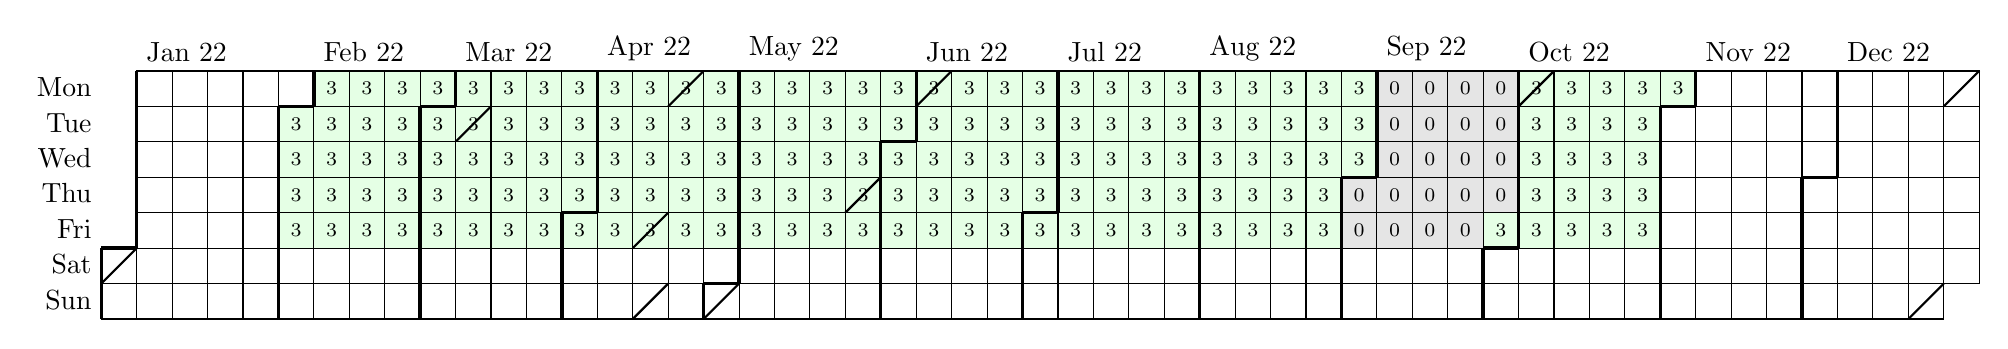
\begin{tikzpicture}[xscale=0.45,yscale=0.45]
\node[above left] at (0,6) {Mon};
\node[above left] at (0,5) {Tue};
\node[above left] at (0,4) {Wed};
\node[above left] at (0,3) {Thu};
\node[above left] at (0,2) {Fri};
\node[above left] at (0,1) {Sat};
\node[above left] at (0,0) {Sun};
\draw[draw=black,thin] (0,1) rectangle (1,2);
\draw[draw=black,very thick] (0,2) -- (1,2);
\draw[draw=black,very thick] (0,1) -- (0,2);
\draw[draw=black,thick] (0,1) -- (1,2);
\draw[draw=black,thin] (0,0) rectangle (1,1);
\draw[draw=black,very thick] (0,0) -- (0,1);
\draw[draw=black,thin] (1,6) rectangle (2,7);
\node[above right] at (1,7) {Jan 22};
\draw[draw=black,very thick] (1,6) -- (1,7);
\draw[draw=black,thin] (1,5) rectangle (2,6);
\draw[draw=black,very thick] (1,5) -- (1,6);
\draw[draw=black,thin] (1,4) rectangle (2,5);
\draw[draw=black,very thick] (1,4) -- (1,5);
\draw[draw=black,thin] (1,3) rectangle (2,4);
\draw[draw=black,very thick] (1,3) -- (1,4);
\draw[draw=black,thin] (1,2) rectangle (2,3);
\draw[draw=black,very thick] (1,2) -- (1,3);
\draw[draw=black,thin] (1,1) rectangle (2,2);
\draw[draw=black,thin] (1,0) rectangle (2,1);
\draw[draw=black,thin] (2,6) rectangle (3,7);
\draw[draw=black,thin] (2,5) rectangle (3,6);
\draw[draw=black,thin] (2,4) rectangle (3,5);
\draw[draw=black,thin] (2,3) rectangle (3,4);
\draw[draw=black,thin] (2,2) rectangle (3,3);
\draw[draw=black,thin] (2,1) rectangle (3,2);
\draw[draw=black,thin] (2,0) rectangle (3,1);
\draw[draw=black,thin] (3,6) rectangle (4,7);
\draw[draw=black,thin] (3,5) rectangle (4,6);
\draw[draw=black,thin] (3,4) rectangle (4,5);
\draw[draw=black,thin] (3,3) rectangle (4,4);
\draw[draw=black,thin] (3,2) rectangle (4,3);
\draw[draw=black,thin] (3,1) rectangle (4,2);
\draw[draw=black,thin] (3,0) rectangle (4,1);
\draw[draw=black,thin] (4,6) rectangle (5,7);
\draw[draw=black,thin] (4,5) rectangle (5,6);
\draw[draw=black,thin] (4,4) rectangle (5,5);
\draw[draw=black,thin] (4,3) rectangle (5,4);
\draw[draw=black,thin] (4,2) rectangle (5,3);
\draw[draw=black,thin] (4,1) rectangle (5,2);
\draw[draw=black,thin] (4,0) rectangle (5,1);
\draw[draw=black,thin] (5,6) rectangle (6,7);
\draw[draw=black,thin,fill=green!10] (5,5) rectangle node[font=\scriptsize] {3} (6,6);
\draw[draw=black,very thick] (5,6) -- (6,6);
\draw[draw=black,very thick] (5,5) -- (5,6);
\draw[draw=black,thin,fill=green!10] (5,4) rectangle node[font=\scriptsize] {3} (6,5);
\draw[draw=black,very thick] (5,4) -- (5,5);
\draw[draw=black,thin,fill=green!10] (5,3) rectangle node[font=\scriptsize] {3} (6,4);
\draw[draw=black,very thick] (5,3) -- (5,4);
\draw[draw=black,thin,fill=green!10] (5,2) rectangle node[font=\scriptsize] {3} (6,3);
\draw[draw=black,very thick] (5,2) -- (5,3);
\draw[draw=black,thin] (5,1) rectangle (6,2);
\draw[draw=black,very thick] (5,1) -- (5,2);
\draw[draw=black,thin] (5,0) rectangle (6,1);
\draw[draw=black,very thick] (5,0) -- (5,1);
\draw[draw=black,thin,fill=green!10] (6,6) rectangle node[font=\scriptsize] {3} (7,7);
\node[above right] at (6,7) {Feb 22};
\draw[draw=black,very thick] (6,6) -- (6,7);
\draw[draw=black,thin,fill=green!10] (6,5) rectangle node[font=\scriptsize] {3} (7,6);
\draw[draw=black,thin,fill=green!10] (6,4) rectangle node[font=\scriptsize] {3} (7,5);
\draw[draw=black,thin,fill=green!10] (6,3) rectangle node[font=\scriptsize] {3} (7,4);
\draw[draw=black,thin,fill=green!10] (6,2) rectangle node[font=\scriptsize] {3} (7,3);
\draw[draw=black,thin] (6,1) rectangle (7,2);
\draw[draw=black,thin] (6,0) rectangle (7,1);
\draw[draw=black,thin,fill=green!10] (7,6) rectangle node[font=\scriptsize] {3} (8,7);
\draw[draw=black,thin,fill=green!10] (7,5) rectangle node[font=\scriptsize] {3} (8,6);
\draw[draw=black,thin,fill=green!10] (7,4) rectangle node[font=\scriptsize] {3} (8,5);
\draw[draw=black,thin,fill=green!10] (7,3) rectangle node[font=\scriptsize] {3} (8,4);
\draw[draw=black,thin,fill=green!10] (7,2) rectangle node[font=\scriptsize] {3} (8,3);
\draw[draw=black,thin] (7,1) rectangle (8,2);
\draw[draw=black,thin] (7,0) rectangle (8,1);
\draw[draw=black,thin,fill=green!10] (8,6) rectangle node[font=\scriptsize] {3} (9,7);
\draw[draw=black,thin,fill=green!10] (8,5) rectangle node[font=\scriptsize] {3} (9,6);
\draw[draw=black,thin,fill=green!10] (8,4) rectangle node[font=\scriptsize] {3} (9,5);
\draw[draw=black,thin,fill=green!10] (8,3) rectangle node[font=\scriptsize] {3} (9,4);
\draw[draw=black,thin,fill=green!10] (8,2) rectangle node[font=\scriptsize] {3} (9,3);
\draw[draw=black,thin] (8,1) rectangle (9,2);
\draw[draw=black,thin] (8,0) rectangle (9,1);
\draw[draw=black,thin,fill=green!10] (9,6) rectangle node[font=\scriptsize] {3} (10,7);
\draw[draw=black,thin,fill=green!10] (9,5) rectangle node[font=\scriptsize] {3} (10,6);
\draw[draw=black,very thick] (9,6) -- (10,6);
\draw[draw=black,very thick] (9,5) -- (9,6);
\draw[draw=black,thin,fill=green!10] (9,4) rectangle node[font=\scriptsize] {3} (10,5);
\draw[draw=black,very thick] (9,4) -- (9,5);
\draw[draw=black,thin,fill=green!10] (9,3) rectangle node[font=\scriptsize] {3} (10,4);
\draw[draw=black,very thick] (9,3) -- (9,4);
\draw[draw=black,thin,fill=green!10] (9,2) rectangle node[font=\scriptsize] {3} (10,3);
\draw[draw=black,very thick] (9,2) -- (9,3);
\draw[draw=black,thin] (9,1) rectangle (10,2);
\draw[draw=black,very thick] (9,1) -- (9,2);
\draw[draw=black,thin] (9,0) rectangle (10,1);
\draw[draw=black,very thick] (9,0) -- (9,1);
\draw[draw=black,thin,fill=green!10] (10,6) rectangle node[font=\scriptsize] {3} (11,7);
\node[above right] at (10,7) {Mar 22};
\draw[draw=black,very thick] (10,6) -- (10,7);
\draw[draw=black,thin,fill=green!10] (10,5) rectangle node[font=\scriptsize] {3} (11,6);
\draw[draw=black,thick] (10,5) -- (11,6);
\draw[draw=black,thin,fill=green!10] (10,4) rectangle node[font=\scriptsize] {3} (11,5);
\draw[draw=black,thin,fill=green!10] (10,3) rectangle node[font=\scriptsize] {3} (11,4);
\draw[draw=black,thin,fill=green!10] (10,2) rectangle node[font=\scriptsize] {3} (11,3);
\draw[draw=black,thin] (10,1) rectangle (11,2);
\draw[draw=black,thin] (10,0) rectangle (11,1);
\draw[draw=black,thin,fill=green!10] (11,6) rectangle node[font=\scriptsize] {3} (12,7);
\draw[draw=black,thin,fill=green!10] (11,5) rectangle node[font=\scriptsize] {3} (12,6);
\draw[draw=black,thin,fill=green!10] (11,4) rectangle node[font=\scriptsize] {3} (12,5);
\draw[draw=black,thin,fill=green!10] (11,3) rectangle node[font=\scriptsize] {3} (12,4);
\draw[draw=black,thin,fill=green!10] (11,2) rectangle node[font=\scriptsize] {3} (12,3);
\draw[draw=black,thin] (11,1) rectangle (12,2);
\draw[draw=black,thin] (11,0) rectangle (12,1);
\draw[draw=black,thin,fill=green!10] (12,6) rectangle node[font=\scriptsize] {3} (13,7);
\draw[draw=black,thin,fill=green!10] (12,5) rectangle node[font=\scriptsize] {3} (13,6);
\draw[draw=black,thin,fill=green!10] (12,4) rectangle node[font=\scriptsize] {3} (13,5);
\draw[draw=black,thin,fill=green!10] (12,3) rectangle node[font=\scriptsize] {3} (13,4);
\draw[draw=black,thin,fill=green!10] (12,2) rectangle node[font=\scriptsize] {3} (13,3);
\draw[draw=black,thin] (12,1) rectangle (13,2);
\draw[draw=black,thin] (12,0) rectangle (13,1);
\draw[draw=black,thin,fill=green!10] (13,6) rectangle node[font=\scriptsize] {3} (14,7);
\draw[draw=black,thin,fill=green!10] (13,5) rectangle node[font=\scriptsize] {3} (14,6);
\draw[draw=black,thin,fill=green!10] (13,4) rectangle node[font=\scriptsize] {3} (14,5);
\draw[draw=black,thin,fill=green!10] (13,3) rectangle node[font=\scriptsize] {3} (14,4);
\draw[draw=black,thin,fill=green!10] (13,2) rectangle node[font=\scriptsize] {3} (14,3);
\draw[draw=black,very thick] (13,3) -- (14,3);
\draw[draw=black,very thick] (13,2) -- (13,3);
\draw[draw=black,thin] (13,1) rectangle (14,2);
\draw[draw=black,very thick] (13,1) -- (13,2);
\draw[draw=black,thin] (13,0) rectangle (14,1);
\draw[draw=black,very thick] (13,0) -- (13,1);
\draw[draw=black,thin,fill=green!10] (14,6) rectangle node[font=\scriptsize] {3} (15,7);
\node[above right] at (14,7) {Apr 22};
\draw[draw=black,very thick] (14,6) -- (14,7);
\draw[draw=black,thin,fill=green!10] (14,5) rectangle node[font=\scriptsize] {3} (15,6);
\draw[draw=black,very thick] (14,5) -- (14,6);
\draw[draw=black,thin,fill=green!10] (14,4) rectangle node[font=\scriptsize] {3} (15,5);
\draw[draw=black,very thick] (14,4) -- (14,5);
\draw[draw=black,thin,fill=green!10] (14,3) rectangle node[font=\scriptsize] {3} (15,4);
\draw[draw=black,very thick] (14,3) -- (14,4);
\draw[draw=black,thin,fill=green!10] (14,2) rectangle node[font=\scriptsize] {3} (15,3);
\draw[draw=black,thin] (14,1) rectangle (15,2);
\draw[draw=black,thin] (14,0) rectangle (15,1);
\draw[draw=black,thin,fill=green!10] (15,6) rectangle node[font=\scriptsize] {3} (16,7);
\draw[draw=black,thin,fill=green!10] (15,5) rectangle node[font=\scriptsize] {3} (16,6);
\draw[draw=black,thin,fill=green!10] (15,4) rectangle node[font=\scriptsize] {3} (16,5);
\draw[draw=black,thin,fill=green!10] (15,3) rectangle node[font=\scriptsize] {3} (16,4);
\draw[draw=black,thin,fill=green!10] (15,2) rectangle node[font=\scriptsize] {3} (16,3);
\draw[draw=black,thick] (15,2) -- (16,3);
\draw[draw=black,thin] (15,1) rectangle (16,2);
\draw[draw=black,thin] (15,0) rectangle (16,1);
\draw[draw=black,thick] (15,0) -- (16,1);
\draw[draw=black,thin,fill=green!10] (16,6) rectangle node[font=\scriptsize] {3} (17,7);
\draw[draw=black,thick] (16,6) -- (17,7);
\draw[draw=black,thin,fill=green!10] (16,5) rectangle node[font=\scriptsize] {3} (17,6);
\draw[draw=black,thin,fill=green!10] (16,4) rectangle node[font=\scriptsize] {3} (17,5);
\draw[draw=black,thin,fill=green!10] (16,3) rectangle node[font=\scriptsize] {3} (17,4);
\draw[draw=black,thin,fill=green!10] (16,2) rectangle node[font=\scriptsize] {3} (17,3);
\draw[draw=black,thin] (16,1) rectangle (17,2);
\draw[draw=black,thin] (16,0) rectangle (17,1);
\draw[draw=black,thin,fill=green!10] (17,6) rectangle node[font=\scriptsize] {3} (18,7);
\draw[draw=black,thin,fill=green!10] (17,5) rectangle node[font=\scriptsize] {3} (18,6);
\draw[draw=black,thin,fill=green!10] (17,4) rectangle node[font=\scriptsize] {3} (18,5);
\draw[draw=black,thin,fill=green!10] (17,3) rectangle node[font=\scriptsize] {3} (18,4);
\draw[draw=black,thin,fill=green!10] (17,2) rectangle node[font=\scriptsize] {3} (18,3);
\draw[draw=black,thin] (17,1) rectangle (18,2);
\draw[draw=black,thin] (17,0) rectangle (18,1);
\draw[draw=black,very thick] (17,1) -- (18,1);
\draw[draw=black,very thick] (17,0) -- (17,1);
\draw[draw=black,thick] (17,0) -- (18,1);
\draw[draw=black,thin,fill=green!10] (18,6) rectangle node[font=\scriptsize] {3} (19,7);
\node[above right] at (18,7) {May 22};
\draw[draw=black,very thick] (18,6) -- (18,7);
\draw[draw=black,thin,fill=green!10] (18,5) rectangle node[font=\scriptsize] {3} (19,6);
\draw[draw=black,very thick] (18,5) -- (18,6);
\draw[draw=black,thin,fill=green!10] (18,4) rectangle node[font=\scriptsize] {3} (19,5);
\draw[draw=black,very thick] (18,4) -- (18,5);
\draw[draw=black,thin,fill=green!10] (18,3) rectangle node[font=\scriptsize] {3} (19,4);
\draw[draw=black,very thick] (18,3) -- (18,4);
\draw[draw=black,thin,fill=green!10] (18,2) rectangle node[font=\scriptsize] {3} (19,3);
\draw[draw=black,very thick] (18,2) -- (18,3);
\draw[draw=black,thin] (18,1) rectangle (19,2);
\draw[draw=black,very thick] (18,1) -- (18,2);
\draw[draw=black,thin] (18,0) rectangle (19,1);
\draw[draw=black,thin,fill=green!10] (19,6) rectangle node[font=\scriptsize] {3} (20,7);
\draw[draw=black,thin,fill=green!10] (19,5) rectangle node[font=\scriptsize] {3} (20,6);
\draw[draw=black,thin,fill=green!10] (19,4) rectangle node[font=\scriptsize] {3} (20,5);
\draw[draw=black,thin,fill=green!10] (19,3) rectangle node[font=\scriptsize] {3} (20,4);
\draw[draw=black,thin,fill=green!10] (19,2) rectangle node[font=\scriptsize] {3} (20,3);
\draw[draw=black,thin] (19,1) rectangle (20,2);
\draw[draw=black,thin] (19,0) rectangle (20,1);
\draw[draw=black,thin,fill=green!10] (20,6) rectangle node[font=\scriptsize] {3} (21,7);
\draw[draw=black,thin,fill=green!10] (20,5) rectangle node[font=\scriptsize] {3} (21,6);
\draw[draw=black,thin,fill=green!10] (20,4) rectangle node[font=\scriptsize] {3} (21,5);
\draw[draw=black,thin,fill=green!10] (20,3) rectangle node[font=\scriptsize] {3} (21,4);
\draw[draw=black,thin,fill=green!10] (20,2) rectangle node[font=\scriptsize] {3} (21,3);
\draw[draw=black,thin] (20,1) rectangle (21,2);
\draw[draw=black,thin] (20,0) rectangle (21,1);
\draw[draw=black,thin,fill=green!10] (21,6) rectangle node[font=\scriptsize] {3} (22,7);
\draw[draw=black,thin,fill=green!10] (21,5) rectangle node[font=\scriptsize] {3} (22,6);
\draw[draw=black,thin,fill=green!10] (21,4) rectangle node[font=\scriptsize] {3} (22,5);
\draw[draw=black,thin,fill=green!10] (21,3) rectangle node[font=\scriptsize] {3} (22,4);
\draw[draw=black,thick] (21,3) -- (22,4);
\draw[draw=black,thin,fill=green!10] (21,2) rectangle node[font=\scriptsize] {3} (22,3);
\draw[draw=black,thin] (21,1) rectangle (22,2);
\draw[draw=black,thin] (21,0) rectangle (22,1);
\draw[draw=black,thin,fill=green!10] (22,6) rectangle node[font=\scriptsize] {3} (23,7);
\draw[draw=black,thin,fill=green!10] (22,5) rectangle node[font=\scriptsize] {3} (23,6);
\draw[draw=black,thin,fill=green!10] (22,4) rectangle node[font=\scriptsize] {3} (23,5);
\draw[draw=black,very thick] (22,5) -- (23,5);
\draw[draw=black,very thick] (22,4) -- (22,5);
\draw[draw=black,thin,fill=green!10] (22,3) rectangle node[font=\scriptsize] {3} (23,4);
\draw[draw=black,very thick] (22,3) -- (22,4);
\draw[draw=black,thin,fill=green!10] (22,2) rectangle node[font=\scriptsize] {3} (23,3);
\draw[draw=black,very thick] (22,2) -- (22,3);
\draw[draw=black,thin] (22,1) rectangle (23,2);
\draw[draw=black,very thick] (22,1) -- (22,2);
\draw[draw=black,thin] (22,0) rectangle (23,1);
\draw[draw=black,very thick] (22,0) -- (22,1);
\draw[draw=black,thin,fill=green!10] (23,6) rectangle node[font=\scriptsize] {3} (24,7);
\node[above right] at (23,7) {Jun 22};
\draw[draw=black,very thick] (23,6) -- (23,7);
\draw[draw=black,thick] (23,6) -- (24,7);
\draw[draw=black,thin,fill=green!10] (23,5) rectangle node[font=\scriptsize] {3} (24,6);
\draw[draw=black,very thick] (23,5) -- (23,6);
\draw[draw=black,thin,fill=green!10] (23,4) rectangle node[font=\scriptsize] {3} (24,5);
\draw[draw=black,thin,fill=green!10] (23,3) rectangle node[font=\scriptsize] {3} (24,4);
\draw[draw=black,thin,fill=green!10] (23,2) rectangle node[font=\scriptsize] {3} (24,3);
\draw[draw=black,thin] (23,1) rectangle (24,2);
\draw[draw=black,thin] (23,0) rectangle (24,1);
\draw[draw=black,thin,fill=green!10] (24,6) rectangle node[font=\scriptsize] {3} (25,7);
\draw[draw=black,thin,fill=green!10] (24,5) rectangle node[font=\scriptsize] {3} (25,6);
\draw[draw=black,thin,fill=green!10] (24,4) rectangle node[font=\scriptsize] {3} (25,5);
\draw[draw=black,thin,fill=green!10] (24,3) rectangle node[font=\scriptsize] {3} (25,4);
\draw[draw=black,thin,fill=green!10] (24,2) rectangle node[font=\scriptsize] {3} (25,3);
\draw[draw=black,thin] (24,1) rectangle (25,2);
\draw[draw=black,thin] (24,0) rectangle (25,1);
\draw[draw=black,thin,fill=green!10] (25,6) rectangle node[font=\scriptsize] {3} (26,7);
\draw[draw=black,thin,fill=green!10] (25,5) rectangle node[font=\scriptsize] {3} (26,6);
\draw[draw=black,thin,fill=green!10] (25,4) rectangle node[font=\scriptsize] {3} (26,5);
\draw[draw=black,thin,fill=green!10] (25,3) rectangle node[font=\scriptsize] {3} (26,4);
\draw[draw=black,thin,fill=green!10] (25,2) rectangle node[font=\scriptsize] {3} (26,3);
\draw[draw=black,thin] (25,1) rectangle (26,2);
\draw[draw=black,thin] (25,0) rectangle (26,1);
\draw[draw=black,thin,fill=green!10] (26,6) rectangle node[font=\scriptsize] {3} (27,7);
\draw[draw=black,thin,fill=green!10] (26,5) rectangle node[font=\scriptsize] {3} (27,6);
\draw[draw=black,thin,fill=green!10] (26,4) rectangle node[font=\scriptsize] {3} (27,5);
\draw[draw=black,thin,fill=green!10] (26,3) rectangle node[font=\scriptsize] {3} (27,4);
\draw[draw=black,thin,fill=green!10] (26,2) rectangle node[font=\scriptsize] {3} (27,3);
\draw[draw=black,very thick] (26,3) -- (27,3);
\draw[draw=black,very thick] (26,2) -- (26,3);
\draw[draw=black,thin] (26,1) rectangle (27,2);
\draw[draw=black,very thick] (26,1) -- (26,2);
\draw[draw=black,thin] (26,0) rectangle (27,1);
\draw[draw=black,very thick] (26,0) -- (26,1);
\draw[draw=black,thin,fill=green!10] (27,6) rectangle node[font=\scriptsize] {3} (28,7);
\node[above right] at (27,7) {Jul 22};
\draw[draw=black,very thick] (27,6) -- (27,7);
\draw[draw=black,thin,fill=green!10] (27,5) rectangle node[font=\scriptsize] {3} (28,6);
\draw[draw=black,very thick] (27,5) -- (27,6);
\draw[draw=black,thin,fill=green!10] (27,4) rectangle node[font=\scriptsize] {3} (28,5);
\draw[draw=black,very thick] (27,4) -- (27,5);
\draw[draw=black,thin,fill=green!10] (27,3) rectangle node[font=\scriptsize] {3} (28,4);
\draw[draw=black,very thick] (27,3) -- (27,4);
\draw[draw=black,thin,fill=green!10] (27,2) rectangle node[font=\scriptsize] {3} (28,3);
\draw[draw=black,thin] (27,1) rectangle (28,2);
\draw[draw=black,thin] (27,0) rectangle (28,1);
\draw[draw=black,thin,fill=green!10] (28,6) rectangle node[font=\scriptsize] {3} (29,7);
\draw[draw=black,thin,fill=green!10] (28,5) rectangle node[font=\scriptsize] {3} (29,6);
\draw[draw=black,thin,fill=green!10] (28,4) rectangle node[font=\scriptsize] {3} (29,5);
\draw[draw=black,thin,fill=green!10] (28,3) rectangle node[font=\scriptsize] {3} (29,4);
\draw[draw=black,thin,fill=green!10] (28,2) rectangle node[font=\scriptsize] {3} (29,3);
\draw[draw=black,thin] (28,1) rectangle (29,2);
\draw[draw=black,thin] (28,0) rectangle (29,1);
\draw[draw=black,thin,fill=green!10] (29,6) rectangle node[font=\scriptsize] {3} (30,7);
\draw[draw=black,thin,fill=green!10] (29,5) rectangle node[font=\scriptsize] {3} (30,6);
\draw[draw=black,thin,fill=green!10] (29,4) rectangle node[font=\scriptsize] {3} (30,5);
\draw[draw=black,thin,fill=green!10] (29,3) rectangle node[font=\scriptsize] {3} (30,4);
\draw[draw=black,thin,fill=green!10] (29,2) rectangle node[font=\scriptsize] {3} (30,3);
\draw[draw=black,thin] (29,1) rectangle (30,2);
\draw[draw=black,thin] (29,0) rectangle (30,1);
\draw[draw=black,thin,fill=green!10] (30,6) rectangle node[font=\scriptsize] {3} (31,7);
\draw[draw=black,thin,fill=green!10] (30,5) rectangle node[font=\scriptsize] {3} (31,6);
\draw[draw=black,thin,fill=green!10] (30,4) rectangle node[font=\scriptsize] {3} (31,5);
\draw[draw=black,thin,fill=green!10] (30,3) rectangle node[font=\scriptsize] {3} (31,4);
\draw[draw=black,thin,fill=green!10] (30,2) rectangle node[font=\scriptsize] {3} (31,3);
\draw[draw=black,thin] (30,1) rectangle (31,2);
\draw[draw=black,thin] (30,0) rectangle (31,1);
\draw[draw=black,thin,fill=green!10] (31,6) rectangle node[font=\scriptsize] {3} (32,7);
\node[above right] at (31,7) {Aug 22};
\draw[draw=black,very thick] (31,6) -- (31,7);
\draw[draw=black,thin,fill=green!10] (31,5) rectangle node[font=\scriptsize] {3} (32,6);
\draw[draw=black,very thick] (31,5) -- (31,6);
\draw[draw=black,thin,fill=green!10] (31,4) rectangle node[font=\scriptsize] {3} (32,5);
\draw[draw=black,very thick] (31,4) -- (31,5);
\draw[draw=black,thin,fill=green!10] (31,3) rectangle node[font=\scriptsize] {3} (32,4);
\draw[draw=black,very thick] (31,3) -- (31,4);
\draw[draw=black,thin,fill=green!10] (31,2) rectangle node[font=\scriptsize] {3} (32,3);
\draw[draw=black,very thick] (31,2) -- (31,3);
\draw[draw=black,thin] (31,1) rectangle (32,2);
\draw[draw=black,very thick] (31,1) -- (31,2);
\draw[draw=black,thin] (31,0) rectangle (32,1);
\draw[draw=black,very thick] (31,0) -- (31,1);
\draw[draw=black,thin,fill=green!10] (32,6) rectangle node[font=\scriptsize] {3} (33,7);
\draw[draw=black,thin,fill=green!10] (32,5) rectangle node[font=\scriptsize] {3} (33,6);
\draw[draw=black,thin,fill=green!10] (32,4) rectangle node[font=\scriptsize] {3} (33,5);
\draw[draw=black,thin,fill=green!10] (32,3) rectangle node[font=\scriptsize] {3} (33,4);
\draw[draw=black,thin,fill=green!10] (32,2) rectangle node[font=\scriptsize] {3} (33,3);
\draw[draw=black,thin] (32,1) rectangle (33,2);
\draw[draw=black,thin] (32,0) rectangle (33,1);
\draw[draw=black,thin,fill=green!10] (33,6) rectangle node[font=\scriptsize] {3} (34,7);
\draw[draw=black,thin,fill=green!10] (33,5) rectangle node[font=\scriptsize] {3} (34,6);
\draw[draw=black,thin,fill=green!10] (33,4) rectangle node[font=\scriptsize] {3} (34,5);
\draw[draw=black,thin,fill=green!10] (33,3) rectangle node[font=\scriptsize] {3} (34,4);
\draw[draw=black,thin,fill=green!10] (33,2) rectangle node[font=\scriptsize] {3} (34,3);
\draw[draw=black,thin] (33,1) rectangle (34,2);
\draw[draw=black,thin] (33,0) rectangle (34,1);
\draw[draw=black,thin,fill=green!10] (34,6) rectangle node[font=\scriptsize] {3} (35,7);
\draw[draw=black,thin,fill=green!10] (34,5) rectangle node[font=\scriptsize] {3} (35,6);
\draw[draw=black,thin,fill=green!10] (34,4) rectangle node[font=\scriptsize] {3} (35,5);
\draw[draw=black,thin,fill=green!10] (34,3) rectangle node[font=\scriptsize] {3} (35,4);
\draw[draw=black,thin,fill=green!10] (34,2) rectangle node[font=\scriptsize] {3} (35,3);
\draw[draw=black,thin] (34,1) rectangle (35,2);
\draw[draw=black,thin] (34,0) rectangle (35,1);
\draw[draw=black,thin,fill=green!10] (35,6) rectangle node[font=\scriptsize] {3} (36,7);
\draw[draw=black,thin,fill=green!10] (35,5) rectangle node[font=\scriptsize] {3} (36,6);
\draw[draw=black,thin,fill=green!10] (35,4) rectangle node[font=\scriptsize] {3} (36,5);
\draw[draw=black,thin,fill=black!10] (35,3) rectangle node[font=\scriptsize] {0} (36,4);
\draw[draw=black,very thick] (35,4) -- (36,4);
\draw[draw=black,very thick] (35,3) -- (35,4);
\draw[draw=black,thin,fill=black!10] (35,2) rectangle node[font=\scriptsize] {0} (36,3);
\draw[draw=black,very thick] (35,2) -- (35,3);
\draw[draw=black,thin] (35,1) rectangle (36,2);
\draw[draw=black,very thick] (35,1) -- (35,2);
\draw[draw=black,thin] (35,0) rectangle (36,1);
\draw[draw=black,very thick] (35,0) -- (35,1);
\draw[draw=black,thin,fill=black!10] (36,6) rectangle node[font=\scriptsize] {0} (37,7);
\node[above right] at (36,7) {Sep 22};
\draw[draw=black,very thick] (36,6) -- (36,7);
\draw[draw=black,thin,fill=black!10] (36,5) rectangle node[font=\scriptsize] {0} (37,6);
\draw[draw=black,very thick] (36,5) -- (36,6);
\draw[draw=black,thin,fill=black!10] (36,4) rectangle node[font=\scriptsize] {0} (37,5);
\draw[draw=black,very thick] (36,4) -- (36,5);
\draw[draw=black,thin,fill=black!10] (36,3) rectangle node[font=\scriptsize] {0} (37,4);
\draw[draw=black,thin,fill=black!10] (36,2) rectangle node[font=\scriptsize] {0} (37,3);
\draw[draw=black,thin] (36,1) rectangle (37,2);
\draw[draw=black,thin] (36,0) rectangle (37,1);
\draw[draw=black,thin,fill=black!10] (37,6) rectangle node[font=\scriptsize] {0} (38,7);
\draw[draw=black,thin,fill=black!10] (37,5) rectangle node[font=\scriptsize] {0} (38,6);
\draw[draw=black,thin,fill=black!10] (37,4) rectangle node[font=\scriptsize] {0} (38,5);
\draw[draw=black,thin,fill=black!10] (37,3) rectangle node[font=\scriptsize] {0} (38,4);
\draw[draw=black,thin,fill=black!10] (37,2) rectangle node[font=\scriptsize] {0} (38,3);
\draw[draw=black,thin] (37,1) rectangle (38,2);
\draw[draw=black,thin] (37,0) rectangle (38,1);
\draw[draw=black,thin,fill=black!10] (38,6) rectangle node[font=\scriptsize] {0} (39,7);
\draw[draw=black,thin,fill=black!10] (38,5) rectangle node[font=\scriptsize] {0} (39,6);
\draw[draw=black,thin,fill=black!10] (38,4) rectangle node[font=\scriptsize] {0} (39,5);
\draw[draw=black,thin,fill=black!10] (38,3) rectangle node[font=\scriptsize] {0} (39,4);
\draw[draw=black,thin,fill=black!10] (38,2) rectangle node[font=\scriptsize] {0} (39,3);
\draw[draw=black,thin] (38,1) rectangle (39,2);
\draw[draw=black,thin] (38,0) rectangle (39,1);
\draw[draw=black,thin,fill=black!10] (39,6) rectangle node[font=\scriptsize] {0} (40,7);
\draw[draw=black,thin,fill=black!10] (39,5) rectangle node[font=\scriptsize] {0} (40,6);
\draw[draw=black,thin,fill=black!10] (39,4) rectangle node[font=\scriptsize] {0} (40,5);
\draw[draw=black,thin,fill=black!10] (39,3) rectangle node[font=\scriptsize] {0} (40,4);
\draw[draw=black,thin,fill=green!10] (39,2) rectangle node[font=\scriptsize] {3} (40,3);
\draw[draw=black,thin] (39,1) rectangle (40,2);
\draw[draw=black,very thick] (39,2) -- (40,2);
\draw[draw=black,very thick] (39,1) -- (39,2);
\draw[draw=black,thin] (39,0) rectangle (40,1);
\draw[draw=black,very thick] (39,0) -- (39,1);
\draw[draw=black,thin,fill=green!10] (40,6) rectangle node[font=\scriptsize] {3} (41,7);
\node[above right] at (40,7) {Oct 22};
\draw[draw=black,very thick] (40,6) -- (40,7);
\draw[draw=black,thick] (40,6) -- (41,7);
\draw[draw=black,thin,fill=green!10] (40,5) rectangle node[font=\scriptsize] {3} (41,6);
\draw[draw=black,very thick] (40,5) -- (40,6);
\draw[draw=black,thin,fill=green!10] (40,4) rectangle node[font=\scriptsize] {3} (41,5);
\draw[draw=black,very thick] (40,4) -- (40,5);
\draw[draw=black,thin,fill=green!10] (40,3) rectangle node[font=\scriptsize] {3} (41,4);
\draw[draw=black,very thick] (40,3) -- (40,4);
\draw[draw=black,thin,fill=green!10] (40,2) rectangle node[font=\scriptsize] {3} (41,3);
\draw[draw=black,very thick] (40,2) -- (40,3);
\draw[draw=black,thin] (40,1) rectangle (41,2);
\draw[draw=black,thin] (40,0) rectangle (41,1);
\draw[draw=black,thin,fill=green!10] (41,6) rectangle node[font=\scriptsize] {3} (42,7);
\draw[draw=black,thin,fill=green!10] (41,5) rectangle node[font=\scriptsize] {3} (42,6);
\draw[draw=black,thin,fill=green!10] (41,4) rectangle node[font=\scriptsize] {3} (42,5);
\draw[draw=black,thin,fill=green!10] (41,3) rectangle node[font=\scriptsize] {3} (42,4);
\draw[draw=black,thin,fill=green!10] (41,2) rectangle node[font=\scriptsize] {3} (42,3);
\draw[draw=black,thin] (41,1) rectangle (42,2);
\draw[draw=black,thin] (41,0) rectangle (42,1);
\draw[draw=black,thin,fill=green!10] (42,6) rectangle node[font=\scriptsize] {3} (43,7);
\draw[draw=black,thin,fill=green!10] (42,5) rectangle node[font=\scriptsize] {3} (43,6);
\draw[draw=black,thin,fill=green!10] (42,4) rectangle node[font=\scriptsize] {3} (43,5);
\draw[draw=black,thin,fill=green!10] (42,3) rectangle node[font=\scriptsize] {3} (43,4);
\draw[draw=black,thin,fill=green!10] (42,2) rectangle node[font=\scriptsize] {3} (43,3);
\draw[draw=black,thin] (42,1) rectangle (43,2);
\draw[draw=black,thin] (42,0) rectangle (43,1);
\draw[draw=black,thin,fill=green!10] (43,6) rectangle node[font=\scriptsize] {3} (44,7);
\draw[draw=black,thin,fill=green!10] (43,5) rectangle node[font=\scriptsize] {3} (44,6);
\draw[draw=black,thin,fill=green!10] (43,4) rectangle node[font=\scriptsize] {3} (44,5);
\draw[draw=black,thin,fill=green!10] (43,3) rectangle node[font=\scriptsize] {3} (44,4);
\draw[draw=black,thin,fill=green!10] (43,2) rectangle node[font=\scriptsize] {3} (44,3);
\draw[draw=black,thin] (43,1) rectangle (44,2);
\draw[draw=black,thin] (43,0) rectangle (44,1);
\draw[draw=black,thin,fill=green!10] (44,6) rectangle node[font=\scriptsize] {3} (45,7);
\draw[draw=black,thin] (44,5) rectangle (45,6);
\draw[draw=black,very thick] (44,6) -- (45,6);
\draw[draw=black,very thick] (44,5) -- (44,6);
\draw[draw=black,thin] (44,4) rectangle (45,5);
\draw[draw=black,very thick] (44,4) -- (44,5);
\draw[draw=black,thin] (44,3) rectangle (45,4);
\draw[draw=black,very thick] (44,3) -- (44,4);
\draw[draw=black,thin] (44,2) rectangle (45,3);
\draw[draw=black,very thick] (44,2) -- (44,3);
\draw[draw=black,thin] (44,1) rectangle (45,2);
\draw[draw=black,very thick] (44,1) -- (44,2);
\draw[draw=black,thin] (44,0) rectangle (45,1);
\draw[draw=black,very thick] (44,0) -- (44,1);
\draw[draw=black,thin] (45,6) rectangle (46,7);
\node[above right] at (45,7) {Nov 22};
\draw[draw=black,very thick] (45,6) -- (45,7);
\draw[draw=black,thin] (45,5) rectangle (46,6);
\draw[draw=black,thin] (45,4) rectangle (46,5);
\draw[draw=black,thin] (45,3) rectangle (46,4);
\draw[draw=black,thin] (45,2) rectangle (46,3);
\draw[draw=black,thin] (45,1) rectangle (46,2);
\draw[draw=black,thin] (45,0) rectangle (46,1);
\draw[draw=black,thin] (46,6) rectangle (47,7);
\draw[draw=black,thin] (46,5) rectangle (47,6);
\draw[draw=black,thin] (46,4) rectangle (47,5);
\draw[draw=black,thin] (46,3) rectangle (47,4);
\draw[draw=black,thin] (46,2) rectangle (47,3);
\draw[draw=black,thin] (46,1) rectangle (47,2);
\draw[draw=black,thin] (46,0) rectangle (47,1);
\draw[draw=black,thin] (47,6) rectangle (48,7);
\draw[draw=black,thin] (47,5) rectangle (48,6);
\draw[draw=black,thin] (47,4) rectangle (48,5);
\draw[draw=black,thin] (47,3) rectangle (48,4);
\draw[draw=black,thin] (47,2) rectangle (48,3);
\draw[draw=black,thin] (47,1) rectangle (48,2);
\draw[draw=black,thin] (47,0) rectangle (48,1);
\draw[draw=black,thin] (48,6) rectangle (49,7);
\draw[draw=black,thin] (48,5) rectangle (49,6);
\draw[draw=black,thin] (48,4) rectangle (49,5);
\draw[draw=black,thin] (48,3) rectangle (49,4);
\draw[draw=black,very thick] (48,4) -- (49,4);
\draw[draw=black,very thick] (48,3) -- (48,4);
\draw[draw=black,thin] (48,2) rectangle (49,3);
\draw[draw=black,very thick] (48,2) -- (48,3);
\draw[draw=black,thin] (48,1) rectangle (49,2);
\draw[draw=black,very thick] (48,1) -- (48,2);
\draw[draw=black,thin] (48,0) rectangle (49,1);
\draw[draw=black,very thick] (48,0) -- (48,1);
\draw[draw=black,thin] (49,6) rectangle (50,7);
\node[above right] at (49,7) {Dec 22};
\draw[draw=black,very thick] (49,6) -- (49,7);
\draw[draw=black,thin] (49,5) rectangle (50,6);
\draw[draw=black,very thick] (49,5) -- (49,6);
\draw[draw=black,thin] (49,4) rectangle (50,5);
\draw[draw=black,very thick] (49,4) -- (49,5);
\draw[draw=black,thin] (49,3) rectangle (50,4);
\draw[draw=black,thin] (49,2) rectangle (50,3);
\draw[draw=black,thin] (49,1) rectangle (50,2);
\draw[draw=black,thin] (49,0) rectangle (50,1);
\draw[draw=black,thin] (50,6) rectangle (51,7);
\draw[draw=black,thin] (50,5) rectangle (51,6);
\draw[draw=black,thin] (50,4) rectangle (51,5);
\draw[draw=black,thin] (50,3) rectangle (51,4);
\draw[draw=black,thin] (50,2) rectangle (51,3);
\draw[draw=black,thin] (50,1) rectangle (51,2);
\draw[draw=black,thin] (50,0) rectangle (51,1);
\draw[draw=black,thin] (51,6) rectangle (52,7);
\draw[draw=black,thin] (51,5) rectangle (52,6);
\draw[draw=black,thin] (51,4) rectangle (52,5);
\draw[draw=black,thin] (51,3) rectangle (52,4);
\draw[draw=black,thin] (51,2) rectangle (52,3);
\draw[draw=black,thin] (51,1) rectangle (52,2);
\draw[draw=black,thin] (51,0) rectangle (52,1);
\draw[draw=black,thick] (51,0) -- (52,1);
\draw[draw=black,thin] (52,6) rectangle (53,7);
\draw[draw=black,thick] (52,6) -- (53,7);
\draw[draw=black,thin] (52,5) rectangle (53,6);
\draw[draw=black,thin] (52,4) rectangle (53,5);
\draw[draw=black,thin] (52,3) rectangle (53,4);
\draw[draw=black,thin] (52,2) rectangle (53,3);
\draw[draw=black,thin] (52,1) rectangle (53,2);
\end{tikzpicture}
}
\begin{itemize}
\item Resulting shift calendar
\end{itemize}

\end{frame}

\begin{frame}
\frametitle{Weekly Machine Dependent Calendar}
\scalebox{0.4}{
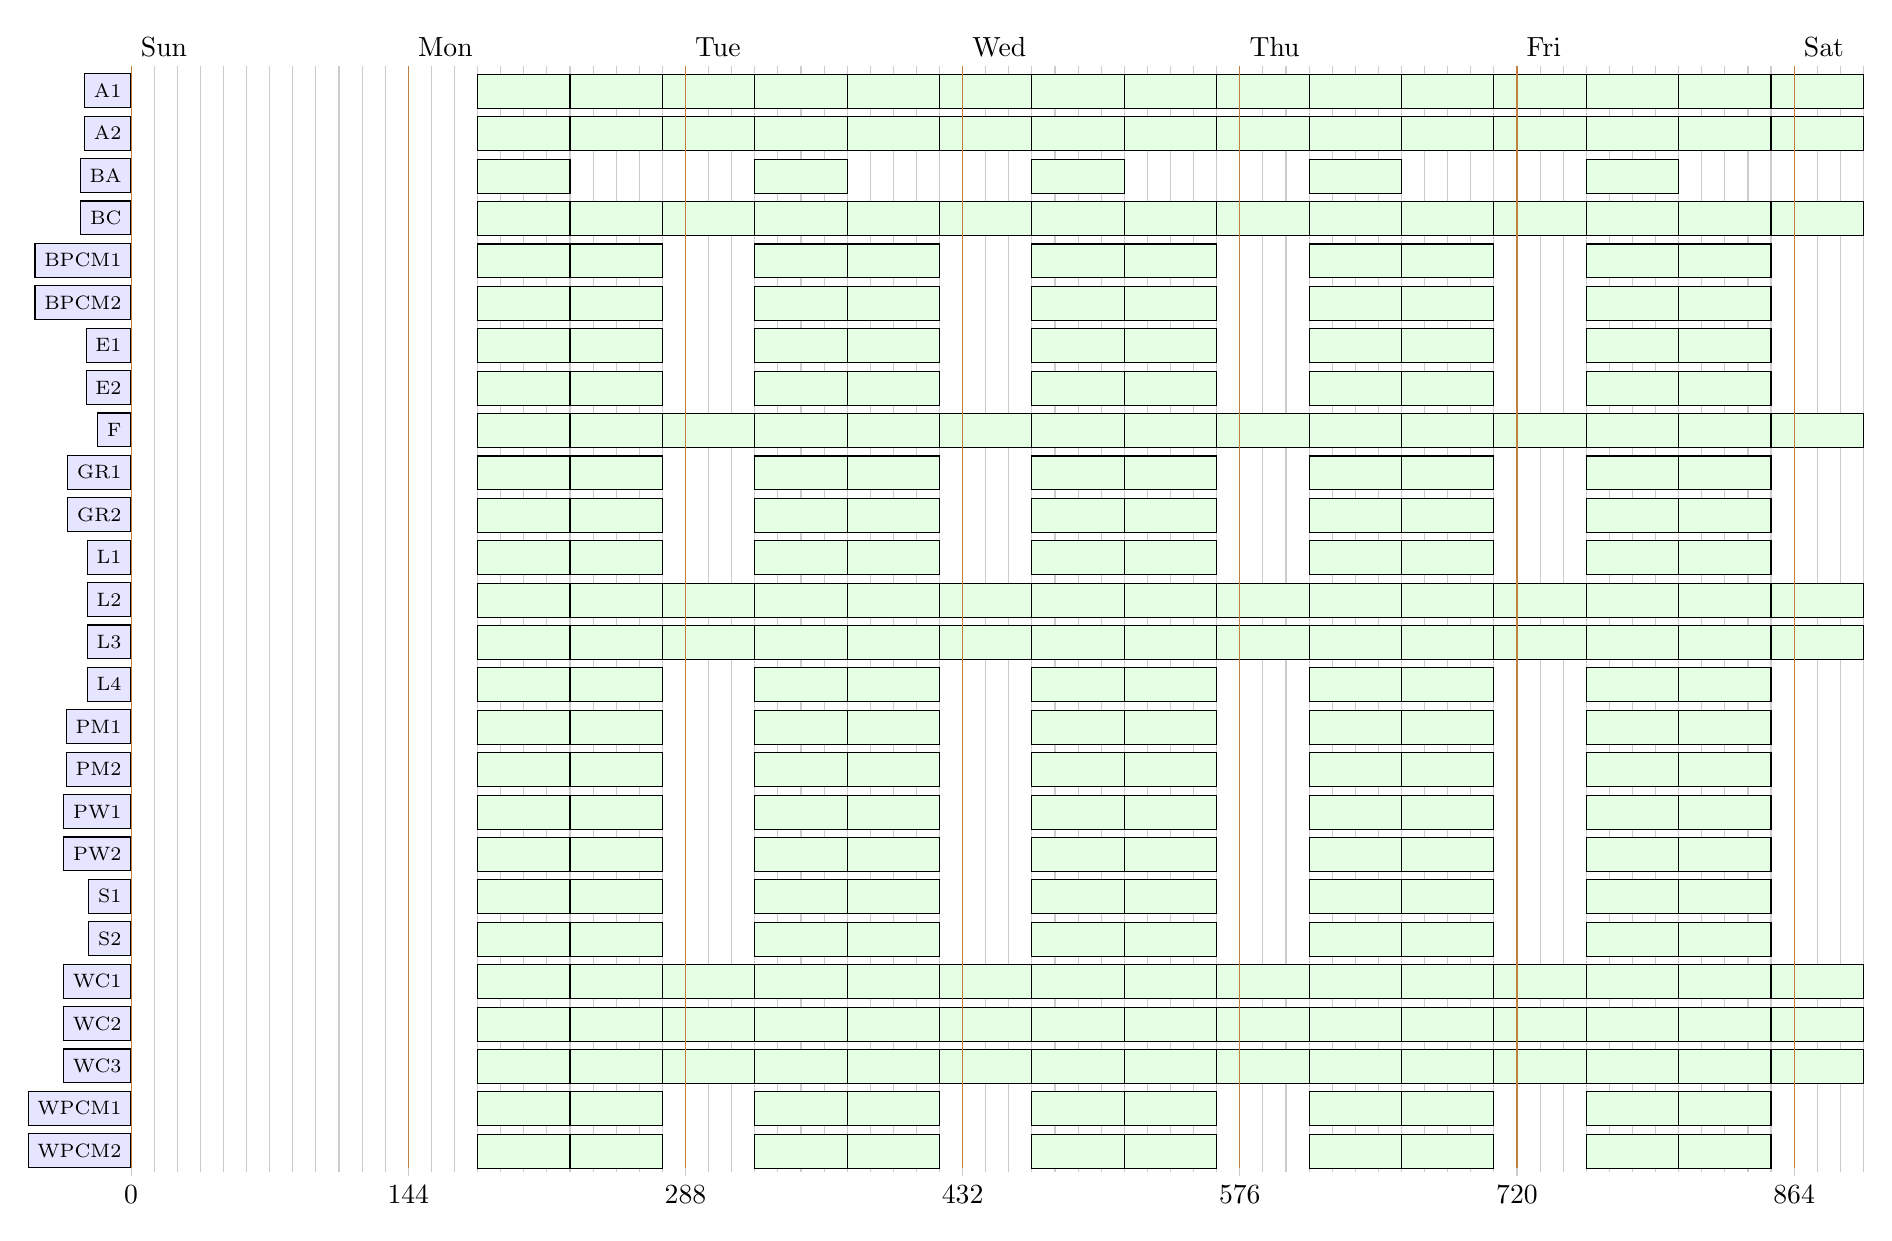
\begin{tikzpicture}[xscale=1.000000,yscale=1.000000]
\draw[draw=black!20] (0.000000,14.000000) -- (0.000000,-0.100000);
\node[below] at (0.000000,-0.100000) {0};
\draw[draw=black!20] (3.520000,14.000000) -- (3.520000,-0.100000);
\node[below] at (3.520000,-0.100000) {144};
\draw[draw=black!20] (7.040000,14.000000) -- (7.040000,-0.100000);
\node[below] at (7.040000,-0.100000) {288};
\draw[draw=black!20] (10.560000,14.000000) -- (10.560000,-0.100000);
\node[below] at (10.560000,-0.100000) {432};
\draw[draw=black!20] (14.080000,14.000000) -- (14.080000,-0.100000);
\node[below] at (14.080000,-0.100000) {576};
\draw[draw=black!20] (17.600000,14.000000) -- (17.600000,-0.100000);
\node[below] at (17.600000,-0.100000) {720};
\draw[draw=black!20] (21.120000,14.000000) -- (21.120000,-0.100000);
\node[below] at (21.120000,-0.100000) {864};
\draw[draw=black!20] (0.000000,14.000000) -- (0.000000,-0.050000);
\draw[draw=black!20] (0.293333,14.000000) -- (0.293333,-0.050000);
\draw[draw=black!20] (0.586667,14.000000) -- (0.586667,-0.050000);
\draw[draw=black!20] (0.880000,14.000000) -- (0.880000,-0.050000);
\draw[draw=black!20] (1.173333,14.000000) -- (1.173333,-0.050000);
\draw[draw=black!20] (1.466667,14.000000) -- (1.466667,-0.050000);
\draw[draw=black!20] (1.760000,14.000000) -- (1.760000,-0.050000);
\draw[draw=black!20] (2.053333,14.000000) -- (2.053333,-0.050000);
\draw[draw=black!20] (2.346667,14.000000) -- (2.346667,-0.050000);
\draw[draw=black!20] (2.640000,14.000000) -- (2.640000,-0.050000);
\draw[draw=black!20] (2.933333,14.000000) -- (2.933333,-0.050000);
\draw[draw=black!20] (3.226667,14.000000) -- (3.226667,-0.050000);
\draw[draw=black!20] (3.520000,14.000000) -- (3.520000,-0.050000);
\draw[draw=black!20] (3.813333,14.000000) -- (3.813333,-0.050000);
\draw[draw=black!20] (4.106667,14.000000) -- (4.106667,-0.050000);
\draw[draw=black!20] (4.400000,14.000000) -- (4.400000,-0.050000);
\draw[draw=black!20] (4.693333,14.000000) -- (4.693333,-0.050000);
\draw[draw=black!20] (4.986667,14.000000) -- (4.986667,-0.050000);
\draw[draw=black!20] (5.280000,14.000000) -- (5.280000,-0.050000);
\draw[draw=black!20] (5.573333,14.000000) -- (5.573333,-0.050000);
\draw[draw=black!20] (5.866667,14.000000) -- (5.866667,-0.050000);
\draw[draw=black!20] (6.160000,14.000000) -- (6.160000,-0.050000);
\draw[draw=black!20] (6.453333,14.000000) -- (6.453333,-0.050000);
\draw[draw=black!20] (6.746667,14.000000) -- (6.746667,-0.050000);
\draw[draw=black!20] (7.040000,14.000000) -- (7.040000,-0.050000);
\draw[draw=black!20] (7.333333,14.000000) -- (7.333333,-0.050000);
\draw[draw=black!20] (7.626667,14.000000) -- (7.626667,-0.050000);
\draw[draw=black!20] (7.920000,14.000000) -- (7.920000,-0.050000);
\draw[draw=black!20] (8.213333,14.000000) -- (8.213333,-0.050000);
\draw[draw=black!20] (8.506667,14.000000) -- (8.506667,-0.050000);
\draw[draw=black!20] (8.800000,14.000000) -- (8.800000,-0.050000);
\draw[draw=black!20] (9.093333,14.000000) -- (9.093333,-0.050000);
\draw[draw=black!20] (9.386667,14.000000) -- (9.386667,-0.050000);
\draw[draw=black!20] (9.680000,14.000000) -- (9.680000,-0.050000);
\draw[draw=black!20] (9.973333,14.000000) -- (9.973333,-0.050000);
\draw[draw=black!20] (10.266667,14.000000) -- (10.266667,-0.050000);
\draw[draw=black!20] (10.560000,14.000000) -- (10.560000,-0.050000);
\draw[draw=black!20] (10.853333,14.000000) -- (10.853333,-0.050000);
\draw[draw=black!20] (11.146667,14.000000) -- (11.146667,-0.050000);
\draw[draw=black!20] (11.440000,14.000000) -- (11.440000,-0.050000);
\draw[draw=black!20] (11.733333,14.000000) -- (11.733333,-0.050000);
\draw[draw=black!20] (12.026667,14.000000) -- (12.026667,-0.050000);
\draw[draw=black!20] (12.320000,14.000000) -- (12.320000,-0.050000);
\draw[draw=black!20] (12.613333,14.000000) -- (12.613333,-0.050000);
\draw[draw=black!20] (12.906667,14.000000) -- (12.906667,-0.050000);
\draw[draw=black!20] (13.200000,14.000000) -- (13.200000,-0.050000);
\draw[draw=black!20] (13.493333,14.000000) -- (13.493333,-0.050000);
\draw[draw=black!20] (13.786667,14.000000) -- (13.786667,-0.050000);
\draw[draw=black!20] (14.080000,14.000000) -- (14.080000,-0.050000);
\draw[draw=black!20] (14.373333,14.000000) -- (14.373333,-0.050000);
\draw[draw=black!20] (14.666667,14.000000) -- (14.666667,-0.050000);
\draw[draw=black!20] (14.960000,14.000000) -- (14.960000,-0.050000);
\draw[draw=black!20] (15.253333,14.000000) -- (15.253333,-0.050000);
\draw[draw=black!20] (15.546667,14.000000) -- (15.546667,-0.050000);
\draw[draw=black!20] (15.840000,14.000000) -- (15.840000,-0.050000);
\draw[draw=black!20] (16.133333,14.000000) -- (16.133333,-0.050000);
\draw[draw=black!20] (16.426667,14.000000) -- (16.426667,-0.050000);
\draw[draw=black!20] (16.720000,14.000000) -- (16.720000,-0.050000);
\draw[draw=black!20] (17.013333,14.000000) -- (17.013333,-0.050000);
\draw[draw=black!20] (17.306667,14.000000) -- (17.306667,-0.050000);
\draw[draw=black!20] (17.600000,14.000000) -- (17.600000,-0.050000);
\draw[draw=black!20] (17.893333,14.000000) -- (17.893333,-0.050000);
\draw[draw=black!20] (18.186667,14.000000) -- (18.186667,-0.050000);
\draw[draw=black!20] (18.480000,14.000000) -- (18.480000,-0.050000);
\draw[draw=black!20] (18.773333,14.000000) -- (18.773333,-0.050000);
\draw[draw=black!20] (19.066667,14.000000) -- (19.066667,-0.050000);
\draw[draw=black!20] (19.360000,14.000000) -- (19.360000,-0.050000);
\draw[draw=black!20] (19.653333,14.000000) -- (19.653333,-0.050000);
\draw[draw=black!20] (19.946667,14.000000) -- (19.946667,-0.050000);
\draw[draw=black!20] (20.240000,14.000000) -- (20.240000,-0.050000);
\draw[draw=black!20] (20.533333,14.000000) -- (20.533333,-0.050000);
\draw[draw=black!20] (20.826667,14.000000) -- (20.826667,-0.050000);
\draw[draw=black!20] (21.120000,14.000000) -- (21.120000,-0.050000);
\draw[draw=black!20] (21.413333,14.000000) -- (21.413333,-0.050000);
\draw[draw=black!20] (21.706667,14.000000) -- (21.706667,-0.050000);
\draw[draw=black!20] (22.000000,14.000000) -- (22.000000,-0.050000);
\node[draw=black,fill=blue!10,font=\scriptsize,minimum height=0.430769cm,above left] (WPCM2) at (0,0.000000) {WPCM2};
\node[draw=black,fill=blue!10,font=\scriptsize,minimum height=0.430769cm,above left] (WPCM1) at (0,0.538462) {WPCM1};
\node[draw=black,fill=blue!10,font=\scriptsize,minimum height=0.430769cm,above left] (WC3) at (0,1.076923) {WC3};
\node[draw=black,fill=blue!10,font=\scriptsize,minimum height=0.430769cm,above left] (WC2) at (0,1.615385) {WC2};
\node[draw=black,fill=blue!10,font=\scriptsize,minimum height=0.430769cm,above left] (WC1) at (0,2.153846) {WC1};
\node[draw=black,fill=blue!10,font=\scriptsize,minimum height=0.430769cm,above left] (S2) at (0,2.692308) {S2};
\node[draw=black,fill=blue!10,font=\scriptsize,minimum height=0.430769cm,above left] (S1) at (0,3.230769) {S1};
\node[draw=black,fill=blue!10,font=\scriptsize,minimum height=0.430769cm,above left] (PW2) at (0,3.769231) {PW2};
\node[draw=black,fill=blue!10,font=\scriptsize,minimum height=0.430769cm,above left] (PW1) at (0,4.307692) {PW1};
\node[draw=black,fill=blue!10,font=\scriptsize,minimum height=0.430769cm,above left] (PM2) at (0,4.846154) {PM2};
\node[draw=black,fill=blue!10,font=\scriptsize,minimum height=0.430769cm,above left] (PM1) at (0,5.384615) {PM1};
\node[draw=black,fill=blue!10,font=\scriptsize,minimum height=0.430769cm,above left] (L4) at (0,5.923077) {L4};
\node[draw=black,fill=blue!10,font=\scriptsize,minimum height=0.430769cm,above left] (L3) at (0,6.461538) {L3};
\node[draw=black,fill=blue!10,font=\scriptsize,minimum height=0.430769cm,above left] (L2) at (0,7.000000) {L2};
\node[draw=black,fill=blue!10,font=\scriptsize,minimum height=0.430769cm,above left] (L1) at (0,7.538462) {L1};
\node[draw=black,fill=blue!10,font=\scriptsize,minimum height=0.430769cm,above left] (GR2) at (0,8.076923) {GR2};
\node[draw=black,fill=blue!10,font=\scriptsize,minimum height=0.430769cm,above left] (GR1) at (0,8.615385) {GR1};
\node[draw=black,fill=blue!10,font=\scriptsize,minimum height=0.430769cm,above left] (F) at (0,9.153846) {F};
\node[draw=black,fill=blue!10,font=\scriptsize,minimum height=0.430769cm,above left] (E2) at (0,9.692308) {E2};
\node[draw=black,fill=blue!10,font=\scriptsize,minimum height=0.430769cm,above left] (E1) at (0,10.230769) {E1};
\node[draw=black,fill=blue!10,font=\scriptsize,minimum height=0.430769cm,above left] (BPCM2) at (0,10.769231) {BPCM2};
\node[draw=black,fill=blue!10,font=\scriptsize,minimum height=0.430769cm,above left] (BPCM1) at (0,11.307692) {BPCM1};
\node[draw=black,fill=blue!10,font=\scriptsize,minimum height=0.430769cm,above left] (BC) at (0,11.846154) {BC};
\node[draw=black,fill=blue!10,font=\scriptsize,minimum height=0.430769cm,above left] (BA) at (0,12.384615) {BA};
\node[draw=black,fill=blue!10,font=\scriptsize,minimum height=0.430769cm,above left] (A2) at (0,12.923077) {A2};
\node[draw=black,fill=blue!10,font=\scriptsize,minimum height=0.430769cm,above left] (A1) at (0,13.461538) {A1};
\draw[draw=black,fill=green!10] (4.400000,13.461538) rectangle node {} (5.573333,13.892308);
\draw[draw=black,fill=green!10] (5.573333,13.461538) rectangle node {} (6.746667,13.892308);
\draw[draw=black,fill=green!10] (6.746667,13.461538) rectangle node {} (7.920000,13.892308);
\draw[draw=black,fill=green!10] (4.400000,12.923077) rectangle node {} (5.573333,13.353846);
\draw[draw=black,fill=green!10] (5.573333,12.923077) rectangle node {} (6.746667,13.353846);
\draw[draw=black,fill=green!10] (6.746667,12.923077) rectangle node {} (7.920000,13.353846);
\draw[draw=black,fill=green!10] (4.400000,7.538462) rectangle node {} (5.573333,7.969231);
\draw[draw=black,fill=green!10] (5.573333,7.538462) rectangle node {} (6.746667,7.969231);
\draw[draw=black,fill=green!10] (4.400000,7.000000) rectangle node {} (5.573333,7.430769);
\draw[draw=black,fill=green!10] (5.573333,7.000000) rectangle node {} (6.746667,7.430769);
\draw[draw=black,fill=green!10] (6.746667,7.000000) rectangle node {} (7.920000,7.430769);
\draw[draw=black,fill=green!10] (4.400000,6.461538) rectangle node {} (5.573333,6.892308);
\draw[draw=black,fill=green!10] (5.573333,6.461538) rectangle node {} (6.746667,6.892308);
\draw[draw=black,fill=green!10] (6.746667,6.461538) rectangle node {} (7.920000,6.892308);
\draw[draw=black,fill=green!10] (4.400000,5.923077) rectangle node {} (5.573333,6.353846);
\draw[draw=black,fill=green!10] (5.573333,5.923077) rectangle node {} (6.746667,6.353846);
\draw[draw=black,fill=green!10] (4.400000,10.230769) rectangle node {} (5.573333,10.661538);
\draw[draw=black,fill=green!10] (5.573333,10.230769) rectangle node {} (6.746667,10.661538);
\draw[draw=black,fill=green!10] (4.400000,9.692308) rectangle node {} (5.573333,10.123077);
\draw[draw=black,fill=green!10] (5.573333,9.692308) rectangle node {} (6.746667,10.123077);
\draw[draw=black,fill=green!10] (4.400000,3.230769) rectangle node {} (5.573333,3.661538);
\draw[draw=black,fill=green!10] (5.573333,3.230769) rectangle node {} (6.746667,3.661538);
\draw[draw=black,fill=green!10] (4.400000,2.692308) rectangle node {} (5.573333,3.123077);
\draw[draw=black,fill=green!10] (5.573333,2.692308) rectangle node {} (6.746667,3.123077);
\draw[draw=black,fill=green!10] (4.400000,12.384615) rectangle node {} (5.573333,12.815385);
\draw[draw=black,fill=green!10] (4.400000,2.153846) rectangle node {} (5.573333,2.584615);
\draw[draw=black,fill=green!10] (5.573333,2.153846) rectangle node {} (6.746667,2.584615);
\draw[draw=black,fill=green!10] (6.746667,2.153846) rectangle node {} (7.920000,2.584615);
\draw[draw=black,fill=green!10] (4.400000,1.615385) rectangle node {} (5.573333,2.046154);
\draw[draw=black,fill=green!10] (5.573333,1.615385) rectangle node {} (6.746667,2.046154);
\draw[draw=black,fill=green!10] (6.746667,1.615385) rectangle node {} (7.920000,2.046154);
\draw[draw=black,fill=green!10] (4.400000,1.076923) rectangle node {} (5.573333,1.507692);
\draw[draw=black,fill=green!10] (5.573333,1.076923) rectangle node {} (6.746667,1.507692);
\draw[draw=black,fill=green!10] (6.746667,1.076923) rectangle node {} (7.920000,1.507692);
\draw[draw=black,fill=green!10] (4.400000,11.846154) rectangle node {} (5.573333,12.276923);
\draw[draw=black,fill=green!10] (5.573333,11.846154) rectangle node {} (6.746667,12.276923);
\draw[draw=black,fill=green!10] (6.746667,11.846154) rectangle node {} (7.920000,12.276923);
\draw[draw=black,fill=green!10] (4.400000,9.153846) rectangle node {} (5.573333,9.584615);
\draw[draw=black,fill=green!10] (5.573333,9.153846) rectangle node {} (6.746667,9.584615);
\draw[draw=black,fill=green!10] (6.746667,9.153846) rectangle node {} (7.920000,9.584615);
\draw[draw=black,fill=green!10] (4.400000,5.384615) rectangle node {} (5.573333,5.815385);
\draw[draw=black,fill=green!10] (5.573333,5.384615) rectangle node {} (6.746667,5.815385);
\draw[draw=black,fill=green!10] (4.400000,4.846154) rectangle node {} (5.573333,5.276923);
\draw[draw=black,fill=green!10] (5.573333,4.846154) rectangle node {} (6.746667,5.276923);
\draw[draw=black,fill=green!10] (4.400000,4.307692) rectangle node {} (5.573333,4.738462);
\draw[draw=black,fill=green!10] (5.573333,4.307692) rectangle node {} (6.746667,4.738462);
\draw[draw=black,fill=green!10] (4.400000,3.769231) rectangle node {} (5.573333,4.200000);
\draw[draw=black,fill=green!10] (5.573333,3.769231) rectangle node {} (6.746667,4.200000);
\draw[draw=black,fill=green!10] (4.400000,11.307692) rectangle node {} (5.573333,11.738462);
\draw[draw=black,fill=green!10] (5.573333,11.307692) rectangle node {} (6.746667,11.738462);
\draw[draw=black,fill=green!10] (4.400000,10.769231) rectangle node {} (5.573333,11.200000);
\draw[draw=black,fill=green!10] (5.573333,10.769231) rectangle node {} (6.746667,11.200000);
\draw[draw=black,fill=green!10] (4.400000,0.538462) rectangle node {} (5.573333,0.969231);
\draw[draw=black,fill=green!10] (5.573333,0.538462) rectangle node {} (6.746667,0.969231);
\draw[draw=black,fill=green!10] (4.400000,0.000000) rectangle node {} (5.573333,0.430769);
\draw[draw=black,fill=green!10] (5.573333,0.000000) rectangle node {} (6.746667,0.430769);
\draw[draw=black,fill=green!10] (4.400000,8.615385) rectangle node {} (5.573333,9.046154);
\draw[draw=black,fill=green!10] (5.573333,8.615385) rectangle node {} (6.746667,9.046154);
\draw[draw=black,fill=green!10] (4.400000,8.076923) rectangle node {} (5.573333,8.507692);
\draw[draw=black,fill=green!10] (5.573333,8.076923) rectangle node {} (6.746667,8.507692);
\draw[draw=black,fill=green!10] (7.920000,13.461538) rectangle node {} (9.093333,13.892308);
\draw[draw=black,fill=green!10] (9.093333,13.461538) rectangle node {} (10.266667,13.892308);
\draw[draw=black,fill=green!10] (10.266667,13.461538) rectangle node {} (11.440000,13.892308);
\draw[draw=black,fill=green!10] (7.920000,12.923077) rectangle node {} (9.093333,13.353846);
\draw[draw=black,fill=green!10] (9.093333,12.923077) rectangle node {} (10.266667,13.353846);
\draw[draw=black,fill=green!10] (10.266667,12.923077) rectangle node {} (11.440000,13.353846);
\draw[draw=black,fill=green!10] (7.920000,7.538462) rectangle node {} (9.093333,7.969231);
\draw[draw=black,fill=green!10] (9.093333,7.538462) rectangle node {} (10.266667,7.969231);
\draw[draw=black,fill=green!10] (7.920000,7.000000) rectangle node {} (9.093333,7.430769);
\draw[draw=black,fill=green!10] (9.093333,7.000000) rectangle node {} (10.266667,7.430769);
\draw[draw=black,fill=green!10] (10.266667,7.000000) rectangle node {} (11.440000,7.430769);
\draw[draw=black,fill=green!10] (7.920000,6.461538) rectangle node {} (9.093333,6.892308);
\draw[draw=black,fill=green!10] (9.093333,6.461538) rectangle node {} (10.266667,6.892308);
\draw[draw=black,fill=green!10] (10.266667,6.461538) rectangle node {} (11.440000,6.892308);
\draw[draw=black,fill=green!10] (7.920000,5.923077) rectangle node {} (9.093333,6.353846);
\draw[draw=black,fill=green!10] (9.093333,5.923077) rectangle node {} (10.266667,6.353846);
\draw[draw=black,fill=green!10] (7.920000,10.230769) rectangle node {} (9.093333,10.661538);
\draw[draw=black,fill=green!10] (9.093333,10.230769) rectangle node {} (10.266667,10.661538);
\draw[draw=black,fill=green!10] (7.920000,9.692308) rectangle node {} (9.093333,10.123077);
\draw[draw=black,fill=green!10] (9.093333,9.692308) rectangle node {} (10.266667,10.123077);
\draw[draw=black,fill=green!10] (7.920000,3.230769) rectangle node {} (9.093333,3.661538);
\draw[draw=black,fill=green!10] (9.093333,3.230769) rectangle node {} (10.266667,3.661538);
\draw[draw=black,fill=green!10] (7.920000,2.692308) rectangle node {} (9.093333,3.123077);
\draw[draw=black,fill=green!10] (9.093333,2.692308) rectangle node {} (10.266667,3.123077);
\draw[draw=black,fill=green!10] (7.920000,12.384615) rectangle node {} (9.093333,12.815385);
\draw[draw=black,fill=green!10] (7.920000,2.153846) rectangle node {} (9.093333,2.584615);
\draw[draw=black,fill=green!10] (9.093333,2.153846) rectangle node {} (10.266667,2.584615);
\draw[draw=black,fill=green!10] (10.266667,2.153846) rectangle node {} (11.440000,2.584615);
\draw[draw=black,fill=green!10] (7.920000,1.615385) rectangle node {} (9.093333,2.046154);
\draw[draw=black,fill=green!10] (9.093333,1.615385) rectangle node {} (10.266667,2.046154);
\draw[draw=black,fill=green!10] (10.266667,1.615385) rectangle node {} (11.440000,2.046154);
\draw[draw=black,fill=green!10] (7.920000,1.076923) rectangle node {} (9.093333,1.507692);
\draw[draw=black,fill=green!10] (9.093333,1.076923) rectangle node {} (10.266667,1.507692);
\draw[draw=black,fill=green!10] (10.266667,1.076923) rectangle node {} (11.440000,1.507692);
\draw[draw=black,fill=green!10] (7.920000,11.846154) rectangle node {} (9.093333,12.276923);
\draw[draw=black,fill=green!10] (9.093333,11.846154) rectangle node {} (10.266667,12.276923);
\draw[draw=black,fill=green!10] (10.266667,11.846154) rectangle node {} (11.440000,12.276923);
\draw[draw=black,fill=green!10] (7.920000,9.153846) rectangle node {} (9.093333,9.584615);
\draw[draw=black,fill=green!10] (9.093333,9.153846) rectangle node {} (10.266667,9.584615);
\draw[draw=black,fill=green!10] (10.266667,9.153846) rectangle node {} (11.440000,9.584615);
\draw[draw=black,fill=green!10] (7.920000,5.384615) rectangle node {} (9.093333,5.815385);
\draw[draw=black,fill=green!10] (9.093333,5.384615) rectangle node {} (10.266667,5.815385);
\draw[draw=black,fill=green!10] (7.920000,4.846154) rectangle node {} (9.093333,5.276923);
\draw[draw=black,fill=green!10] (9.093333,4.846154) rectangle node {} (10.266667,5.276923);
\draw[draw=black,fill=green!10] (7.920000,4.307692) rectangle node {} (9.093333,4.738462);
\draw[draw=black,fill=green!10] (9.093333,4.307692) rectangle node {} (10.266667,4.738462);
\draw[draw=black,fill=green!10] (7.920000,3.769231) rectangle node {} (9.093333,4.200000);
\draw[draw=black,fill=green!10] (9.093333,3.769231) rectangle node {} (10.266667,4.200000);
\draw[draw=black,fill=green!10] (7.920000,11.307692) rectangle node {} (9.093333,11.738462);
\draw[draw=black,fill=green!10] (9.093333,11.307692) rectangle node {} (10.266667,11.738462);
\draw[draw=black,fill=green!10] (7.920000,10.769231) rectangle node {} (9.093333,11.200000);
\draw[draw=black,fill=green!10] (9.093333,10.769231) rectangle node {} (10.266667,11.200000);
\draw[draw=black,fill=green!10] (7.920000,0.538462) rectangle node {} (9.093333,0.969231);
\draw[draw=black,fill=green!10] (9.093333,0.538462) rectangle node {} (10.266667,0.969231);
\draw[draw=black,fill=green!10] (7.920000,0.000000) rectangle node {} (9.093333,0.430769);
\draw[draw=black,fill=green!10] (9.093333,0.000000) rectangle node {} (10.266667,0.430769);
\draw[draw=black,fill=green!10] (7.920000,8.615385) rectangle node {} (9.093333,9.046154);
\draw[draw=black,fill=green!10] (9.093333,8.615385) rectangle node {} (10.266667,9.046154);
\draw[draw=black,fill=green!10] (7.920000,8.076923) rectangle node {} (9.093333,8.507692);
\draw[draw=black,fill=green!10] (9.093333,8.076923) rectangle node {} (10.266667,8.507692);
\draw[draw=black,fill=green!10] (11.440000,13.461538) rectangle node {} (12.613333,13.892308);
\draw[draw=black,fill=green!10] (12.613333,13.461538) rectangle node {} (13.786667,13.892308);
\draw[draw=black,fill=green!10] (13.786667,13.461538) rectangle node {} (14.960000,13.892308);
\draw[draw=black,fill=green!10] (11.440000,12.923077) rectangle node {} (12.613333,13.353846);
\draw[draw=black,fill=green!10] (12.613333,12.923077) rectangle node {} (13.786667,13.353846);
\draw[draw=black,fill=green!10] (13.786667,12.923077) rectangle node {} (14.960000,13.353846);
\draw[draw=black,fill=green!10] (11.440000,7.538462) rectangle node {} (12.613333,7.969231);
\draw[draw=black,fill=green!10] (12.613333,7.538462) rectangle node {} (13.786667,7.969231);
\draw[draw=black,fill=green!10] (11.440000,7.000000) rectangle node {} (12.613333,7.430769);
\draw[draw=black,fill=green!10] (12.613333,7.000000) rectangle node {} (13.786667,7.430769);
\draw[draw=black,fill=green!10] (13.786667,7.000000) rectangle node {} (14.960000,7.430769);
\draw[draw=black,fill=green!10] (11.440000,6.461538) rectangle node {} (12.613333,6.892308);
\draw[draw=black,fill=green!10] (12.613333,6.461538) rectangle node {} (13.786667,6.892308);
\draw[draw=black,fill=green!10] (13.786667,6.461538) rectangle node {} (14.960000,6.892308);
\draw[draw=black,fill=green!10] (11.440000,5.923077) rectangle node {} (12.613333,6.353846);
\draw[draw=black,fill=green!10] (12.613333,5.923077) rectangle node {} (13.786667,6.353846);
\draw[draw=black,fill=green!10] (11.440000,10.230769) rectangle node {} (12.613333,10.661538);
\draw[draw=black,fill=green!10] (12.613333,10.230769) rectangle node {} (13.786667,10.661538);
\draw[draw=black,fill=green!10] (11.440000,9.692308) rectangle node {} (12.613333,10.123077);
\draw[draw=black,fill=green!10] (12.613333,9.692308) rectangle node {} (13.786667,10.123077);
\draw[draw=black,fill=green!10] (11.440000,3.230769) rectangle node {} (12.613333,3.661538);
\draw[draw=black,fill=green!10] (12.613333,3.230769) rectangle node {} (13.786667,3.661538);
\draw[draw=black,fill=green!10] (11.440000,2.692308) rectangle node {} (12.613333,3.123077);
\draw[draw=black,fill=green!10] (12.613333,2.692308) rectangle node {} (13.786667,3.123077);
\draw[draw=black,fill=green!10] (11.440000,12.384615) rectangle node {} (12.613333,12.815385);
\draw[draw=black,fill=green!10] (11.440000,2.153846) rectangle node {} (12.613333,2.584615);
\draw[draw=black,fill=green!10] (12.613333,2.153846) rectangle node {} (13.786667,2.584615);
\draw[draw=black,fill=green!10] (13.786667,2.153846) rectangle node {} (14.960000,2.584615);
\draw[draw=black,fill=green!10] (11.440000,1.615385) rectangle node {} (12.613333,2.046154);
\draw[draw=black,fill=green!10] (12.613333,1.615385) rectangle node {} (13.786667,2.046154);
\draw[draw=black,fill=green!10] (13.786667,1.615385) rectangle node {} (14.960000,2.046154);
\draw[draw=black,fill=green!10] (11.440000,1.076923) rectangle node {} (12.613333,1.507692);
\draw[draw=black,fill=green!10] (12.613333,1.076923) rectangle node {} (13.786667,1.507692);
\draw[draw=black,fill=green!10] (13.786667,1.076923) rectangle node {} (14.960000,1.507692);
\draw[draw=black,fill=green!10] (11.440000,11.846154) rectangle node {} (12.613333,12.276923);
\draw[draw=black,fill=green!10] (12.613333,11.846154) rectangle node {} (13.786667,12.276923);
\draw[draw=black,fill=green!10] (13.786667,11.846154) rectangle node {} (14.960000,12.276923);
\draw[draw=black,fill=green!10] (11.440000,9.153846) rectangle node {} (12.613333,9.584615);
\draw[draw=black,fill=green!10] (12.613333,9.153846) rectangle node {} (13.786667,9.584615);
\draw[draw=black,fill=green!10] (13.786667,9.153846) rectangle node {} (14.960000,9.584615);
\draw[draw=black,fill=green!10] (11.440000,5.384615) rectangle node {} (12.613333,5.815385);
\draw[draw=black,fill=green!10] (12.613333,5.384615) rectangle node {} (13.786667,5.815385);
\draw[draw=black,fill=green!10] (11.440000,4.846154) rectangle node {} (12.613333,5.276923);
\draw[draw=black,fill=green!10] (12.613333,4.846154) rectangle node {} (13.786667,5.276923);
\draw[draw=black,fill=green!10] (11.440000,4.307692) rectangle node {} (12.613333,4.738462);
\draw[draw=black,fill=green!10] (12.613333,4.307692) rectangle node {} (13.786667,4.738462);
\draw[draw=black,fill=green!10] (11.440000,3.769231) rectangle node {} (12.613333,4.200000);
\draw[draw=black,fill=green!10] (12.613333,3.769231) rectangle node {} (13.786667,4.200000);
\draw[draw=black,fill=green!10] (11.440000,11.307692) rectangle node {} (12.613333,11.738462);
\draw[draw=black,fill=green!10] (12.613333,11.307692) rectangle node {} (13.786667,11.738462);
\draw[draw=black,fill=green!10] (11.440000,10.769231) rectangle node {} (12.613333,11.200000);
\draw[draw=black,fill=green!10] (12.613333,10.769231) rectangle node {} (13.786667,11.200000);
\draw[draw=black,fill=green!10] (11.440000,0.538462) rectangle node {} (12.613333,0.969231);
\draw[draw=black,fill=green!10] (12.613333,0.538462) rectangle node {} (13.786667,0.969231);
\draw[draw=black,fill=green!10] (11.440000,0.000000) rectangle node {} (12.613333,0.430769);
\draw[draw=black,fill=green!10] (12.613333,0.000000) rectangle node {} (13.786667,0.430769);
\draw[draw=black,fill=green!10] (11.440000,8.615385) rectangle node {} (12.613333,9.046154);
\draw[draw=black,fill=green!10] (12.613333,8.615385) rectangle node {} (13.786667,9.046154);
\draw[draw=black,fill=green!10] (11.440000,8.076923) rectangle node {} (12.613333,8.507692);
\draw[draw=black,fill=green!10] (12.613333,8.076923) rectangle node {} (13.786667,8.507692);
\draw[draw=black,fill=green!10] (14.960000,13.461538) rectangle node {} (16.133333,13.892308);
\draw[draw=black,fill=green!10] (16.133333,13.461538) rectangle node {} (17.306667,13.892308);
\draw[draw=black,fill=green!10] (17.306667,13.461538) rectangle node {} (18.480000,13.892308);
\draw[draw=black,fill=green!10] (14.960000,12.923077) rectangle node {} (16.133333,13.353846);
\draw[draw=black,fill=green!10] (16.133333,12.923077) rectangle node {} (17.306667,13.353846);
\draw[draw=black,fill=green!10] (17.306667,12.923077) rectangle node {} (18.480000,13.353846);
\draw[draw=black,fill=green!10] (14.960000,7.538462) rectangle node {} (16.133333,7.969231);
\draw[draw=black,fill=green!10] (16.133333,7.538462) rectangle node {} (17.306667,7.969231);
\draw[draw=black,fill=green!10] (14.960000,7.000000) rectangle node {} (16.133333,7.430769);
\draw[draw=black,fill=green!10] (16.133333,7.000000) rectangle node {} (17.306667,7.430769);
\draw[draw=black,fill=green!10] (17.306667,7.000000) rectangle node {} (18.480000,7.430769);
\draw[draw=black,fill=green!10] (14.960000,6.461538) rectangle node {} (16.133333,6.892308);
\draw[draw=black,fill=green!10] (16.133333,6.461538) rectangle node {} (17.306667,6.892308);
\draw[draw=black,fill=green!10] (17.306667,6.461538) rectangle node {} (18.480000,6.892308);
\draw[draw=black,fill=green!10] (14.960000,5.923077) rectangle node {} (16.133333,6.353846);
\draw[draw=black,fill=green!10] (16.133333,5.923077) rectangle node {} (17.306667,6.353846);
\draw[draw=black,fill=green!10] (14.960000,10.230769) rectangle node {} (16.133333,10.661538);
\draw[draw=black,fill=green!10] (16.133333,10.230769) rectangle node {} (17.306667,10.661538);
\draw[draw=black,fill=green!10] (14.960000,9.692308) rectangle node {} (16.133333,10.123077);
\draw[draw=black,fill=green!10] (16.133333,9.692308) rectangle node {} (17.306667,10.123077);
\draw[draw=black,fill=green!10] (14.960000,3.230769) rectangle node {} (16.133333,3.661538);
\draw[draw=black,fill=green!10] (16.133333,3.230769) rectangle node {} (17.306667,3.661538);
\draw[draw=black,fill=green!10] (14.960000,2.692308) rectangle node {} (16.133333,3.123077);
\draw[draw=black,fill=green!10] (16.133333,2.692308) rectangle node {} (17.306667,3.123077);
\draw[draw=black,fill=green!10] (14.960000,12.384615) rectangle node {} (16.133333,12.815385);
\draw[draw=black,fill=green!10] (14.960000,2.153846) rectangle node {} (16.133333,2.584615);
\draw[draw=black,fill=green!10] (16.133333,2.153846) rectangle node {} (17.306667,2.584615);
\draw[draw=black,fill=green!10] (17.306667,2.153846) rectangle node {} (18.480000,2.584615);
\draw[draw=black,fill=green!10] (14.960000,1.615385) rectangle node {} (16.133333,2.046154);
\draw[draw=black,fill=green!10] (16.133333,1.615385) rectangle node {} (17.306667,2.046154);
\draw[draw=black,fill=green!10] (17.306667,1.615385) rectangle node {} (18.480000,2.046154);
\draw[draw=black,fill=green!10] (14.960000,1.076923) rectangle node {} (16.133333,1.507692);
\draw[draw=black,fill=green!10] (16.133333,1.076923) rectangle node {} (17.306667,1.507692);
\draw[draw=black,fill=green!10] (17.306667,1.076923) rectangle node {} (18.480000,1.507692);
\draw[draw=black,fill=green!10] (14.960000,11.846154) rectangle node {} (16.133333,12.276923);
\draw[draw=black,fill=green!10] (16.133333,11.846154) rectangle node {} (17.306667,12.276923);
\draw[draw=black,fill=green!10] (17.306667,11.846154) rectangle node {} (18.480000,12.276923);
\draw[draw=black,fill=green!10] (14.960000,9.153846) rectangle node {} (16.133333,9.584615);
\draw[draw=black,fill=green!10] (16.133333,9.153846) rectangle node {} (17.306667,9.584615);
\draw[draw=black,fill=green!10] (17.306667,9.153846) rectangle node {} (18.480000,9.584615);
\draw[draw=black,fill=green!10] (14.960000,5.384615) rectangle node {} (16.133333,5.815385);
\draw[draw=black,fill=green!10] (16.133333,5.384615) rectangle node {} (17.306667,5.815385);
\draw[draw=black,fill=green!10] (14.960000,4.846154) rectangle node {} (16.133333,5.276923);
\draw[draw=black,fill=green!10] (16.133333,4.846154) rectangle node {} (17.306667,5.276923);
\draw[draw=black,fill=green!10] (14.960000,4.307692) rectangle node {} (16.133333,4.738462);
\draw[draw=black,fill=green!10] (16.133333,4.307692) rectangle node {} (17.306667,4.738462);
\draw[draw=black,fill=green!10] (14.960000,3.769231) rectangle node {} (16.133333,4.200000);
\draw[draw=black,fill=green!10] (16.133333,3.769231) rectangle node {} (17.306667,4.200000);
\draw[draw=black,fill=green!10] (14.960000,11.307692) rectangle node {} (16.133333,11.738462);
\draw[draw=black,fill=green!10] (16.133333,11.307692) rectangle node {} (17.306667,11.738462);
\draw[draw=black,fill=green!10] (14.960000,10.769231) rectangle node {} (16.133333,11.200000);
\draw[draw=black,fill=green!10] (16.133333,10.769231) rectangle node {} (17.306667,11.200000);
\draw[draw=black,fill=green!10] (14.960000,0.538462) rectangle node {} (16.133333,0.969231);
\draw[draw=black,fill=green!10] (16.133333,0.538462) rectangle node {} (17.306667,0.969231);
\draw[draw=black,fill=green!10] (14.960000,0.000000) rectangle node {} (16.133333,0.430769);
\draw[draw=black,fill=green!10] (16.133333,0.000000) rectangle node {} (17.306667,0.430769);
\draw[draw=black,fill=green!10] (14.960000,8.615385) rectangle node {} (16.133333,9.046154);
\draw[draw=black,fill=green!10] (16.133333,8.615385) rectangle node {} (17.306667,9.046154);
\draw[draw=black,fill=green!10] (14.960000,8.076923) rectangle node {} (16.133333,8.507692);
\draw[draw=black,fill=green!10] (16.133333,8.076923) rectangle node {} (17.306667,8.507692);
\draw[draw=black,fill=green!10] (18.480000,13.461538) rectangle node {} (19.653333,13.892308);
\draw[draw=black,fill=green!10] (19.653333,13.461538) rectangle node {} (20.826667,13.892308);
\draw[draw=black,fill=green!10] (20.826667,13.461538) rectangle node {} (22.000000,13.892308);
\draw[draw=black,fill=green!10] (18.480000,12.923077) rectangle node {} (19.653333,13.353846);
\draw[draw=black,fill=green!10] (19.653333,12.923077) rectangle node {} (20.826667,13.353846);
\draw[draw=black,fill=green!10] (20.826667,12.923077) rectangle node {} (22.000000,13.353846);
\draw[draw=black,fill=green!10] (18.480000,7.538462) rectangle node {} (19.653333,7.969231);
\draw[draw=black,fill=green!10] (19.653333,7.538462) rectangle node {} (20.826667,7.969231);
\draw[draw=black,fill=green!10] (18.480000,7.000000) rectangle node {} (19.653333,7.430769);
\draw[draw=black,fill=green!10] (19.653333,7.000000) rectangle node {} (20.826667,7.430769);
\draw[draw=black,fill=green!10] (20.826667,7.000000) rectangle node {} (22.000000,7.430769);
\draw[draw=black,fill=green!10] (18.480000,6.461538) rectangle node {} (19.653333,6.892308);
\draw[draw=black,fill=green!10] (19.653333,6.461538) rectangle node {} (20.826667,6.892308);
\draw[draw=black,fill=green!10] (20.826667,6.461538) rectangle node {} (22.000000,6.892308);
\draw[draw=black,fill=green!10] (18.480000,5.923077) rectangle node {} (19.653333,6.353846);
\draw[draw=black,fill=green!10] (19.653333,5.923077) rectangle node {} (20.826667,6.353846);
\draw[draw=black,fill=green!10] (18.480000,10.230769) rectangle node {} (19.653333,10.661538);
\draw[draw=black,fill=green!10] (19.653333,10.230769) rectangle node {} (20.826667,10.661538);
\draw[draw=black,fill=green!10] (18.480000,9.692308) rectangle node {} (19.653333,10.123077);
\draw[draw=black,fill=green!10] (19.653333,9.692308) rectangle node {} (20.826667,10.123077);
\draw[draw=black,fill=green!10] (18.480000,3.230769) rectangle node {} (19.653333,3.661538);
\draw[draw=black,fill=green!10] (19.653333,3.230769) rectangle node {} (20.826667,3.661538);
\draw[draw=black,fill=green!10] (18.480000,2.692308) rectangle node {} (19.653333,3.123077);
\draw[draw=black,fill=green!10] (19.653333,2.692308) rectangle node {} (20.826667,3.123077);
\draw[draw=black,fill=green!10] (18.480000,12.384615) rectangle node {} (19.653333,12.815385);
\draw[draw=black,fill=green!10] (18.480000,2.153846) rectangle node {} (19.653333,2.584615);
\draw[draw=black,fill=green!10] (19.653333,2.153846) rectangle node {} (20.826667,2.584615);
\draw[draw=black,fill=green!10] (20.826667,2.153846) rectangle node {} (22.000000,2.584615);
\draw[draw=black,fill=green!10] (18.480000,1.615385) rectangle node {} (19.653333,2.046154);
\draw[draw=black,fill=green!10] (19.653333,1.615385) rectangle node {} (20.826667,2.046154);
\draw[draw=black,fill=green!10] (20.826667,1.615385) rectangle node {} (22.000000,2.046154);
\draw[draw=black,fill=green!10] (18.480000,1.076923) rectangle node {} (19.653333,1.507692);
\draw[draw=black,fill=green!10] (19.653333,1.076923) rectangle node {} (20.826667,1.507692);
\draw[draw=black,fill=green!10] (20.826667,1.076923) rectangle node {} (22.000000,1.507692);
\draw[draw=black,fill=green!10] (18.480000,11.846154) rectangle node {} (19.653333,12.276923);
\draw[draw=black,fill=green!10] (19.653333,11.846154) rectangle node {} (20.826667,12.276923);
\draw[draw=black,fill=green!10] (20.826667,11.846154) rectangle node {} (22.000000,12.276923);
\draw[draw=black,fill=green!10] (18.480000,9.153846) rectangle node {} (19.653333,9.584615);
\draw[draw=black,fill=green!10] (19.653333,9.153846) rectangle node {} (20.826667,9.584615);
\draw[draw=black,fill=green!10] (20.826667,9.153846) rectangle node {} (22.000000,9.584615);
\draw[draw=black,fill=green!10] (18.480000,5.384615) rectangle node {} (19.653333,5.815385);
\draw[draw=black,fill=green!10] (19.653333,5.384615) rectangle node {} (20.826667,5.815385);
\draw[draw=black,fill=green!10] (18.480000,4.846154) rectangle node {} (19.653333,5.276923);
\draw[draw=black,fill=green!10] (19.653333,4.846154) rectangle node {} (20.826667,5.276923);
\draw[draw=black,fill=green!10] (18.480000,4.307692) rectangle node {} (19.653333,4.738462);
\draw[draw=black,fill=green!10] (19.653333,4.307692) rectangle node {} (20.826667,4.738462);
\draw[draw=black,fill=green!10] (18.480000,3.769231) rectangle node {} (19.653333,4.200000);
\draw[draw=black,fill=green!10] (19.653333,3.769231) rectangle node {} (20.826667,4.200000);
\draw[draw=black,fill=green!10] (18.480000,11.307692) rectangle node {} (19.653333,11.738462);
\draw[draw=black,fill=green!10] (19.653333,11.307692) rectangle node {} (20.826667,11.738462);
\draw[draw=black,fill=green!10] (18.480000,10.769231) rectangle node {} (19.653333,11.200000);
\draw[draw=black,fill=green!10] (19.653333,10.769231) rectangle node {} (20.826667,11.200000);
\draw[draw=black,fill=green!10] (18.480000,0.538462) rectangle node {} (19.653333,0.969231);
\draw[draw=black,fill=green!10] (19.653333,0.538462) rectangle node {} (20.826667,0.969231);
\draw[draw=black,fill=green!10] (18.480000,0.000000) rectangle node {} (19.653333,0.430769);
\draw[draw=black,fill=green!10] (19.653333,0.000000) rectangle node {} (20.826667,0.430769);
\draw[draw=black,fill=green!10] (18.480000,8.615385) rectangle node {} (19.653333,9.046154);
\draw[draw=black,fill=green!10] (19.653333,8.615385) rectangle node {} (20.826667,9.046154);
\draw[draw=black,fill=green!10] (18.480000,8.076923) rectangle node {} (19.653333,8.507692);
\draw[draw=black,fill=green!10] (19.653333,8.076923) rectangle node {} (20.826667,8.507692);
\draw[draw=brown] (0.000000,14.000000) -- (0.000000,0.000000);
\node[above right] () at (0.000000,14.000000) {Sun};
\draw[draw=brown] (3.520000,14.000000) -- (3.520000,0.000000);
\node[above right] () at (3.520000,14.000000) {Mon};
\draw[draw=brown] (7.040000,14.000000) -- (7.040000,0.000000);
\node[above right] () at (7.040000,14.000000) {Tue};
\draw[draw=brown] (10.560000,14.000000) -- (10.560000,0.000000);
\node[above right] () at (10.560000,14.000000) {Wed};
\draw[draw=brown] (14.080000,14.000000) -- (14.080000,0.000000);
\node[above right] () at (14.080000,14.000000) {Thu};
\draw[draw=brown] (17.600000,14.000000) -- (17.600000,0.000000);
\node[above right] () at (17.600000,14.000000) {Fri};
\draw[draw=brown] (21.120000,14.000000) -- (21.120000,0.000000);
\node[above right] () at (21.120000,14.000000) {Sat};
\end{tikzpicture}

}
\begin{itemize}
\item Note machines running one shift, two shifts, or three shifts
\end{itemize}

\end{frame}

\begin{frame}
\frametitle{ShiftPattern for Workers}
\scalebox{0.45}{
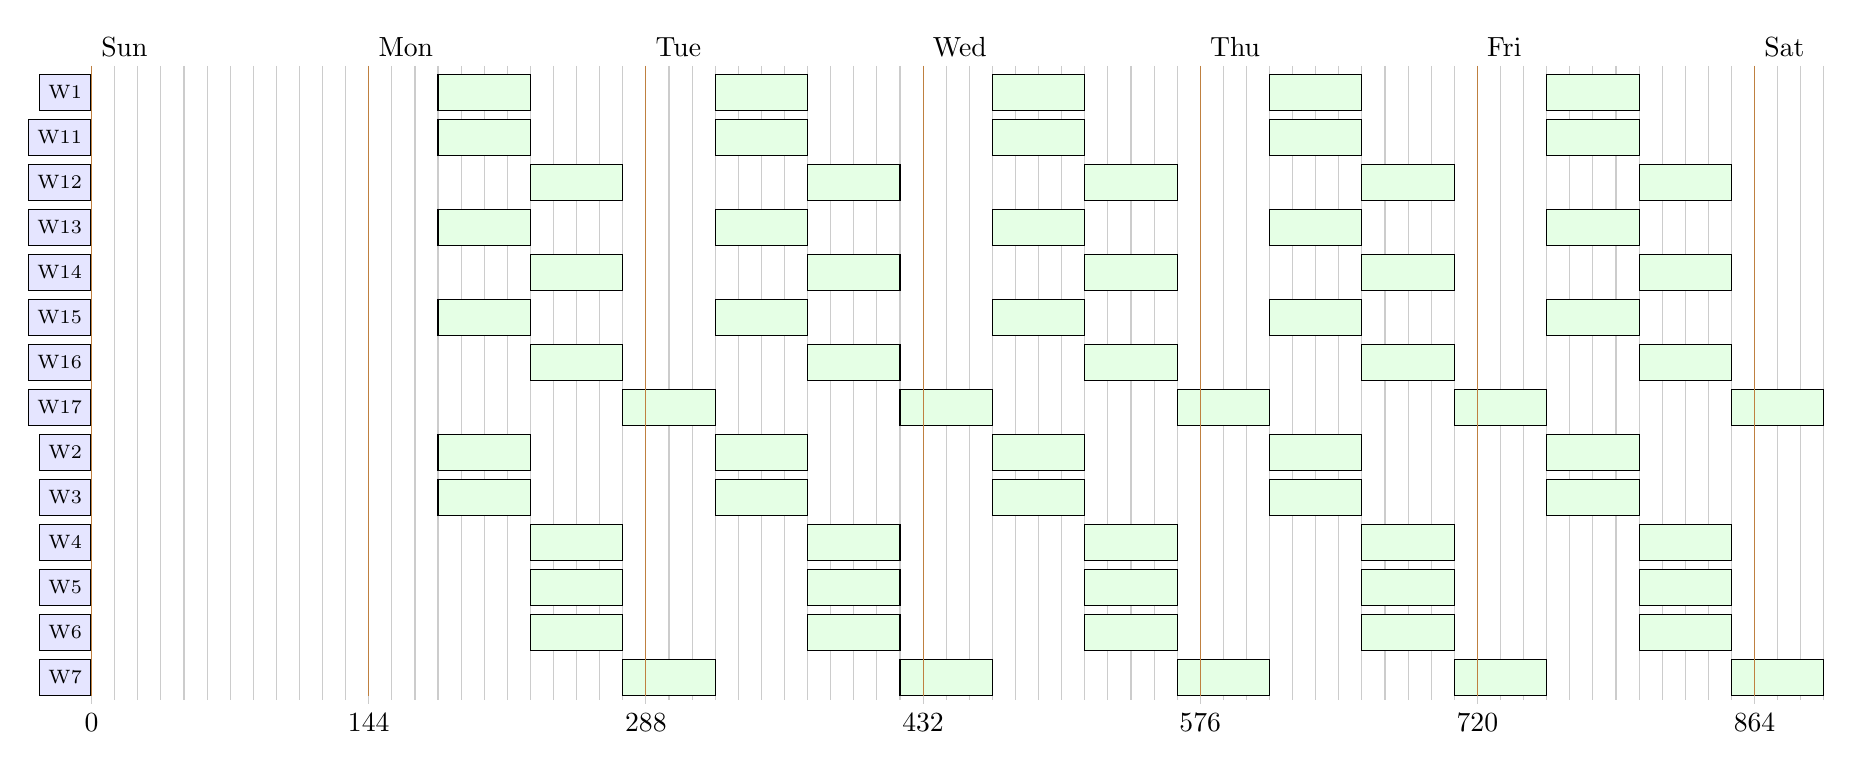
\begin{tikzpicture}[xscale=1.000000,yscale=1.000000]
\draw[draw=black!20] (0.000000,8.000000) -- (0.000000,-0.100000);
\node[below] at (0.000000,-0.100000) {0};
\draw[draw=black!20] (3.520000,8.000000) -- (3.520000,-0.100000);
\node[below] at (3.520000,-0.100000) {144};
\draw[draw=black!20] (7.040000,8.000000) -- (7.040000,-0.100000);
\node[below] at (7.040000,-0.100000) {288};
\draw[draw=black!20] (10.560000,8.000000) -- (10.560000,-0.100000);
\node[below] at (10.560000,-0.100000) {432};
\draw[draw=black!20] (14.080000,8.000000) -- (14.080000,-0.100000);
\node[below] at (14.080000,-0.100000) {576};
\draw[draw=black!20] (17.600000,8.000000) -- (17.600000,-0.100000);
\node[below] at (17.600000,-0.100000) {720};
\draw[draw=black!20] (21.120000,8.000000) -- (21.120000,-0.100000);
\node[below] at (21.120000,-0.100000) {864};
\draw[draw=black!20] (0.000000,8.000000) -- (0.000000,-0.050000);
\draw[draw=black!20] (0.293333,8.000000) -- (0.293333,-0.050000);
\draw[draw=black!20] (0.586667,8.000000) -- (0.586667,-0.050000);
\draw[draw=black!20] (0.880000,8.000000) -- (0.880000,-0.050000);
\draw[draw=black!20] (1.173333,8.000000) -- (1.173333,-0.050000);
\draw[draw=black!20] (1.466667,8.000000) -- (1.466667,-0.050000);
\draw[draw=black!20] (1.760000,8.000000) -- (1.760000,-0.050000);
\draw[draw=black!20] (2.053333,8.000000) -- (2.053333,-0.050000);
\draw[draw=black!20] (2.346667,8.000000) -- (2.346667,-0.050000);
\draw[draw=black!20] (2.640000,8.000000) -- (2.640000,-0.050000);
\draw[draw=black!20] (2.933333,8.000000) -- (2.933333,-0.050000);
\draw[draw=black!20] (3.226667,8.000000) -- (3.226667,-0.050000);
\draw[draw=black!20] (3.520000,8.000000) -- (3.520000,-0.050000);
\draw[draw=black!20] (3.813333,8.000000) -- (3.813333,-0.050000);
\draw[draw=black!20] (4.106667,8.000000) -- (4.106667,-0.050000);
\draw[draw=black!20] (4.400000,8.000000) -- (4.400000,-0.050000);
\draw[draw=black!20] (4.693333,8.000000) -- (4.693333,-0.050000);
\draw[draw=black!20] (4.986667,8.000000) -- (4.986667,-0.050000);
\draw[draw=black!20] (5.280000,8.000000) -- (5.280000,-0.050000);
\draw[draw=black!20] (5.573333,8.000000) -- (5.573333,-0.050000);
\draw[draw=black!20] (5.866667,8.000000) -- (5.866667,-0.050000);
\draw[draw=black!20] (6.160000,8.000000) -- (6.160000,-0.050000);
\draw[draw=black!20] (6.453333,8.000000) -- (6.453333,-0.050000);
\draw[draw=black!20] (6.746667,8.000000) -- (6.746667,-0.050000);
\draw[draw=black!20] (7.040000,8.000000) -- (7.040000,-0.050000);
\draw[draw=black!20] (7.333333,8.000000) -- (7.333333,-0.050000);
\draw[draw=black!20] (7.626667,8.000000) -- (7.626667,-0.050000);
\draw[draw=black!20] (7.920000,8.000000) -- (7.920000,-0.050000);
\draw[draw=black!20] (8.213333,8.000000) -- (8.213333,-0.050000);
\draw[draw=black!20] (8.506667,8.000000) -- (8.506667,-0.050000);
\draw[draw=black!20] (8.800000,8.000000) -- (8.800000,-0.050000);
\draw[draw=black!20] (9.093333,8.000000) -- (9.093333,-0.050000);
\draw[draw=black!20] (9.386667,8.000000) -- (9.386667,-0.050000);
\draw[draw=black!20] (9.680000,8.000000) -- (9.680000,-0.050000);
\draw[draw=black!20] (9.973333,8.000000) -- (9.973333,-0.050000);
\draw[draw=black!20] (10.266667,8.000000) -- (10.266667,-0.050000);
\draw[draw=black!20] (10.560000,8.000000) -- (10.560000,-0.050000);
\draw[draw=black!20] (10.853333,8.000000) -- (10.853333,-0.050000);
\draw[draw=black!20] (11.146667,8.000000) -- (11.146667,-0.050000);
\draw[draw=black!20] (11.440000,8.000000) -- (11.440000,-0.050000);
\draw[draw=black!20] (11.733333,8.000000) -- (11.733333,-0.050000);
\draw[draw=black!20] (12.026667,8.000000) -- (12.026667,-0.050000);
\draw[draw=black!20] (12.320000,8.000000) -- (12.320000,-0.050000);
\draw[draw=black!20] (12.613333,8.000000) -- (12.613333,-0.050000);
\draw[draw=black!20] (12.906667,8.000000) -- (12.906667,-0.050000);
\draw[draw=black!20] (13.200000,8.000000) -- (13.200000,-0.050000);
\draw[draw=black!20] (13.493333,8.000000) -- (13.493333,-0.050000);
\draw[draw=black!20] (13.786667,8.000000) -- (13.786667,-0.050000);
\draw[draw=black!20] (14.080000,8.000000) -- (14.080000,-0.050000);
\draw[draw=black!20] (14.373333,8.000000) -- (14.373333,-0.050000);
\draw[draw=black!20] (14.666667,8.000000) -- (14.666667,-0.050000);
\draw[draw=black!20] (14.960000,8.000000) -- (14.960000,-0.050000);
\draw[draw=black!20] (15.253333,8.000000) -- (15.253333,-0.050000);
\draw[draw=black!20] (15.546667,8.000000) -- (15.546667,-0.050000);
\draw[draw=black!20] (15.840000,8.000000) -- (15.840000,-0.050000);
\draw[draw=black!20] (16.133333,8.000000) -- (16.133333,-0.050000);
\draw[draw=black!20] (16.426667,8.000000) -- (16.426667,-0.050000);
\draw[draw=black!20] (16.720000,8.000000) -- (16.720000,-0.050000);
\draw[draw=black!20] (17.013333,8.000000) -- (17.013333,-0.050000);
\draw[draw=black!20] (17.306667,8.000000) -- (17.306667,-0.050000);
\draw[draw=black!20] (17.600000,8.000000) -- (17.600000,-0.050000);
\draw[draw=black!20] (17.893333,8.000000) -- (17.893333,-0.050000);
\draw[draw=black!20] (18.186667,8.000000) -- (18.186667,-0.050000);
\draw[draw=black!20] (18.480000,8.000000) -- (18.480000,-0.050000);
\draw[draw=black!20] (18.773333,8.000000) -- (18.773333,-0.050000);
\draw[draw=black!20] (19.066667,8.000000) -- (19.066667,-0.050000);
\draw[draw=black!20] (19.360000,8.000000) -- (19.360000,-0.050000);
\draw[draw=black!20] (19.653333,8.000000) -- (19.653333,-0.050000);
\draw[draw=black!20] (19.946667,8.000000) -- (19.946667,-0.050000);
\draw[draw=black!20] (20.240000,8.000000) -- (20.240000,-0.050000);
\draw[draw=black!20] (20.533333,8.000000) -- (20.533333,-0.050000);
\draw[draw=black!20] (20.826667,8.000000) -- (20.826667,-0.050000);
\draw[draw=black!20] (21.120000,8.000000) -- (21.120000,-0.050000);
\draw[draw=black!20] (21.413333,8.000000) -- (21.413333,-0.050000);
\draw[draw=black!20] (21.706667,8.000000) -- (21.706667,-0.050000);
\draw[draw=black!20] (22.000000,8.000000) -- (22.000000,-0.050000);
\node[draw=black,fill=blue!10,font=\scriptsize,minimum height=0.457143cm,above left] (W7) at (0,0.000000) {W7};
\node[draw=black,fill=blue!10,font=\scriptsize,minimum height=0.457143cm,above left] (W6) at (0,0.571429) {W6};
\node[draw=black,fill=blue!10,font=\scriptsize,minimum height=0.457143cm,above left] (W5) at (0,1.142857) {W5};
\node[draw=black,fill=blue!10,font=\scriptsize,minimum height=0.457143cm,above left] (W4) at (0,1.714286) {W4};
\node[draw=black,fill=blue!10,font=\scriptsize,minimum height=0.457143cm,above left] (W3) at (0,2.285714) {W3};
\node[draw=black,fill=blue!10,font=\scriptsize,minimum height=0.457143cm,above left] (W2) at (0,2.857143) {W2};
\node[draw=black,fill=blue!10,font=\scriptsize,minimum height=0.457143cm,above left] (W17) at (0,3.428571) {W17};
\node[draw=black,fill=blue!10,font=\scriptsize,minimum height=0.457143cm,above left] (W16) at (0,4.000000) {W16};
\node[draw=black,fill=blue!10,font=\scriptsize,minimum height=0.457143cm,above left] (W15) at (0,4.571429) {W15};
\node[draw=black,fill=blue!10,font=\scriptsize,minimum height=0.457143cm,above left] (W14) at (0,5.142857) {W14};
\node[draw=black,fill=blue!10,font=\scriptsize,minimum height=0.457143cm,above left] (W13) at (0,5.714286) {W13};
\node[draw=black,fill=blue!10,font=\scriptsize,minimum height=0.457143cm,above left] (W12) at (0,6.285714) {W12};
\node[draw=black,fill=blue!10,font=\scriptsize,minimum height=0.457143cm,above left] (W11) at (0,6.857143) {W11};
\node[draw=black,fill=blue!10,font=\scriptsize,minimum height=0.457143cm,above left] (W1) at (0,7.428571) {W1};
\draw[draw=black,fill=green!10] (4.400000,7.428571) rectangle node {} (5.573333,7.885714);
\draw[draw=black,fill=green!10] (4.400000,2.857143) rectangle node {} (5.573333,3.314286);
\draw[draw=black,fill=green!10] (4.400000,2.285714) rectangle node {} (5.573333,2.742857);
\draw[draw=black,fill=green!10] (5.573333,1.714286) rectangle node {} (6.746667,2.171429);
\draw[draw=black,fill=green!10] (5.573333,1.142857) rectangle node {} (6.746667,1.600000);
\draw[draw=black,fill=green!10] (5.573333,0.571429) rectangle node {} (6.746667,1.028571);
\draw[draw=black,fill=green!10] (6.746667,0.000000) rectangle node {} (7.920000,0.457143);
\draw[draw=black,fill=green!10] (4.400000,6.857143) rectangle node {} (5.573333,7.314286);
\draw[draw=black,fill=green!10] (5.573333,6.285714) rectangle node {} (6.746667,6.742857);
\draw[draw=black,fill=green!10] (4.400000,5.714286) rectangle node {} (5.573333,6.171429);
\draw[draw=black,fill=green!10] (5.573333,5.142857) rectangle node {} (6.746667,5.600000);
\draw[draw=black,fill=green!10] (4.400000,4.571429) rectangle node {} (5.573333,5.028571);
\draw[draw=black,fill=green!10] (5.573333,4.000000) rectangle node {} (6.746667,4.457143);
\draw[draw=black,fill=green!10] (6.746667,3.428571) rectangle node {} (7.920000,3.885714);
\draw[draw=black,fill=green!10] (7.920000,7.428571) rectangle node {} (9.093333,7.885714);
\draw[draw=black,fill=green!10] (7.920000,2.857143) rectangle node {} (9.093333,3.314286);
\draw[draw=black,fill=green!10] (7.920000,2.285714) rectangle node {} (9.093333,2.742857);
\draw[draw=black,fill=green!10] (9.093333,1.714286) rectangle node {} (10.266667,2.171429);
\draw[draw=black,fill=green!10] (9.093333,1.142857) rectangle node {} (10.266667,1.600000);
\draw[draw=black,fill=green!10] (9.093333,0.571429) rectangle node {} (10.266667,1.028571);
\draw[draw=black,fill=green!10] (10.266667,0.000000) rectangle node {} (11.440000,0.457143);
\draw[draw=black,fill=green!10] (7.920000,6.857143) rectangle node {} (9.093333,7.314286);
\draw[draw=black,fill=green!10] (9.093333,6.285714) rectangle node {} (10.266667,6.742857);
\draw[draw=black,fill=green!10] (7.920000,5.714286) rectangle node {} (9.093333,6.171429);
\draw[draw=black,fill=green!10] (9.093333,5.142857) rectangle node {} (10.266667,5.600000);
\draw[draw=black,fill=green!10] (7.920000,4.571429) rectangle node {} (9.093333,5.028571);
\draw[draw=black,fill=green!10] (9.093333,4.000000) rectangle node {} (10.266667,4.457143);
\draw[draw=black,fill=green!10] (10.266667,3.428571) rectangle node {} (11.440000,3.885714);
\draw[draw=black,fill=green!10] (11.440000,7.428571) rectangle node {} (12.613333,7.885714);
\draw[draw=black,fill=green!10] (11.440000,2.857143) rectangle node {} (12.613333,3.314286);
\draw[draw=black,fill=green!10] (11.440000,2.285714) rectangle node {} (12.613333,2.742857);
\draw[draw=black,fill=green!10] (12.613333,1.714286) rectangle node {} (13.786667,2.171429);
\draw[draw=black,fill=green!10] (12.613333,1.142857) rectangle node {} (13.786667,1.600000);
\draw[draw=black,fill=green!10] (12.613333,0.571429) rectangle node {} (13.786667,1.028571);
\draw[draw=black,fill=green!10] (13.786667,0.000000) rectangle node {} (14.960000,0.457143);
\draw[draw=black,fill=green!10] (11.440000,6.857143) rectangle node {} (12.613333,7.314286);
\draw[draw=black,fill=green!10] (12.613333,6.285714) rectangle node {} (13.786667,6.742857);
\draw[draw=black,fill=green!10] (11.440000,5.714286) rectangle node {} (12.613333,6.171429);
\draw[draw=black,fill=green!10] (12.613333,5.142857) rectangle node {} (13.786667,5.600000);
\draw[draw=black,fill=green!10] (11.440000,4.571429) rectangle node {} (12.613333,5.028571);
\draw[draw=black,fill=green!10] (12.613333,4.000000) rectangle node {} (13.786667,4.457143);
\draw[draw=black,fill=green!10] (13.786667,3.428571) rectangle node {} (14.960000,3.885714);
\draw[draw=black,fill=green!10] (14.960000,7.428571) rectangle node {} (16.133333,7.885714);
\draw[draw=black,fill=green!10] (14.960000,2.857143) rectangle node {} (16.133333,3.314286);
\draw[draw=black,fill=green!10] (14.960000,2.285714) rectangle node {} (16.133333,2.742857);
\draw[draw=black,fill=green!10] (16.133333,1.714286) rectangle node {} (17.306667,2.171429);
\draw[draw=black,fill=green!10] (16.133333,1.142857) rectangle node {} (17.306667,1.600000);
\draw[draw=black,fill=green!10] (16.133333,0.571429) rectangle node {} (17.306667,1.028571);
\draw[draw=black,fill=green!10] (17.306667,0.000000) rectangle node {} (18.480000,0.457143);
\draw[draw=black,fill=green!10] (14.960000,6.857143) rectangle node {} (16.133333,7.314286);
\draw[draw=black,fill=green!10] (16.133333,6.285714) rectangle node {} (17.306667,6.742857);
\draw[draw=black,fill=green!10] (14.960000,5.714286) rectangle node {} (16.133333,6.171429);
\draw[draw=black,fill=green!10] (16.133333,5.142857) rectangle node {} (17.306667,5.600000);
\draw[draw=black,fill=green!10] (14.960000,4.571429) rectangle node {} (16.133333,5.028571);
\draw[draw=black,fill=green!10] (16.133333,4.000000) rectangle node {} (17.306667,4.457143);
\draw[draw=black,fill=green!10] (17.306667,3.428571) rectangle node {} (18.480000,3.885714);
\draw[draw=black,fill=green!10] (18.480000,7.428571) rectangle node {} (19.653333,7.885714);
\draw[draw=black,fill=green!10] (18.480000,2.857143) rectangle node {} (19.653333,3.314286);
\draw[draw=black,fill=green!10] (18.480000,2.285714) rectangle node {} (19.653333,2.742857);
\draw[draw=black,fill=green!10] (19.653333,1.714286) rectangle node {} (20.826667,2.171429);
\draw[draw=black,fill=green!10] (19.653333,1.142857) rectangle node {} (20.826667,1.600000);
\draw[draw=black,fill=green!10] (19.653333,0.571429) rectangle node {} (20.826667,1.028571);
\draw[draw=black,fill=green!10] (20.826667,0.000000) rectangle node {} (22.000000,0.457143);
\draw[draw=black,fill=green!10] (18.480000,6.857143) rectangle node {} (19.653333,7.314286);
\draw[draw=black,fill=green!10] (19.653333,6.285714) rectangle node {} (20.826667,6.742857);
\draw[draw=black,fill=green!10] (18.480000,5.714286) rectangle node {} (19.653333,6.171429);
\draw[draw=black,fill=green!10] (19.653333,5.142857) rectangle node {} (20.826667,5.600000);
\draw[draw=black,fill=green!10] (18.480000,4.571429) rectangle node {} (19.653333,5.028571);
\draw[draw=black,fill=green!10] (19.653333,4.000000) rectangle node {} (20.826667,4.457143);
\draw[draw=black,fill=green!10] (20.826667,3.428571) rectangle node {} (22.000000,3.885714);
\draw[draw=brown] (0.000000,8.000000) -- (0.000000,0.000000);
\node[above right] () at (0.000000,8.000000) {Sun};
\draw[draw=brown] (3.520000,8.000000) -- (3.520000,0.000000);
\node[above right] () at (3.520000,8.000000) {Mon};
\draw[draw=brown] (7.040000,8.000000) -- (7.040000,0.000000);
\node[above right] () at (7.040000,8.000000) {Tue};
\draw[draw=brown] (10.560000,8.000000) -- (10.560000,0.000000);
\node[above right] () at (10.560000,8.000000) {Wed};
\draw[draw=brown] (14.080000,8.000000) -- (14.080000,0.000000);
\node[above right] () at (14.080000,8.000000) {Thu};
\draw[draw=brown] (17.600000,8.000000) -- (17.600000,0.000000);
\node[above right] () at (17.600000,8.000000) {Fri};
\draw[draw=brown] (21.120000,8.000000) -- (21.120000,0.000000);
\node[above right] () at (21.120000,8.000000) {Sat};
\end{tikzpicture}

}

\begin{itemize}
\item Note different resource levels for morning, afternoon and night shift
\end{itemize}

\end{frame}

\subsection{Calendar Dependent Duration}

\begin{frame}
\frametitle{Calendar Dependent Duration \navail}
\begin{itemize}
\item In some factories, tasks have different duration depending on when they are run
\item During the night-shift fewer workers are available, tasks like cleaning take longer
\item During holidays, most expert operators are absent, tasks take longer due to less experienced operators
\item For every working period, define a utilization factor to define nominal capacity (0-100\%)
\begin{itemize}
\item Tasks take longer if work capacity is lower
\item Only supported in few solvers (CPO)
\end{itemize}

\end{itemize}
\end{frame}


\subsection{Task/Break Interaction}

\begin{frame}
\frametitle{Tasks Stretching over Shutdown \navail}
\begin{itemize}
\item When a machine does not run continuously, the duration of tasks in wall time may change
\end{itemize}

\scalebox{0.2}{
\begin{tikzpicture}[every node/.style={font=\LARGE}]
\node[left] at (0,-0.5) {Sample Tasks};
\node[left] at (0,2) {Start};
\node[left] at (0,1) {End};
\node[left] at (0,3) {Elapsed Time};
\node[left] at (0,5.5) {Time of Day};
\node[left] at (0,7.5) {Day};

\draw[fill=white] (0,7) rectangle node {Day 1} +(24,1);
\draw[fill=white] (24,7) rectangle node {Day 2} +(24,1);

\draw[fill=white] (0,5) rectangle node {00} +(1,1);
\draw[fill=white] (1,5) rectangle node {01} +(1,1);
\draw[fill=white] (2,5) rectangle node {02} +(1,1);
\draw[fill=white] (3,5) rectangle node {03} +(1,1);
\draw[fill=white] (4,5) rectangle node {04} +(1,1);
\draw[fill=white] (5,5) rectangle node {05} +(1,1);
\draw[fill=insight-royalblue!20] (6,5) rectangle node {06} +(1,1);
\draw[fill=insight-royalblue!20] (7,5) rectangle node {07} +(1,1);
\draw[fill=insight-royalblue!20] (8,5) rectangle node {08} +(1,1);
\draw[fill=insight-royalblue!20] (9,5) rectangle node {09} +(1,1);
\draw[fill=insight-royalblue!20] (10,5) rectangle node {10} +(1,1);
\draw[fill=insight-royalblue!20] (11,5) rectangle node {11} +(1,1);
\draw[fill=insight-royalblue!20] (12,5) rectangle node {12} +(1,1);
\draw[fill=insight-royalblue!20] (13,5) rectangle node {13} +(1,1);
\draw[fill=insight-lime!20] (14,5) rectangle node {14} +(1,1);
\draw[fill=insight-lime!20] (15,5) rectangle node {15} +(1,1);
\draw[fill=insight-lime!20] (16,5) rectangle node {16} +(1,1);
\draw[fill=insight-lime!20] (17,5) rectangle node {17} +(1,1);
\draw[fill=insight-lime!20] (18,5) rectangle node {18} +(1,1);
\draw[fill=insight-lime!20] (19,5) rectangle node {19} +(1,1);
\draw[fill=insight-lime!20] (20,5) rectangle node {20} +(1,1);
\draw[fill=insight-lime!20] (21,5) rectangle node {21} +(1,1);
\draw[fill=white] (22,5) rectangle node {22} +(1,1);
\draw[fill=white] (23,5) rectangle node {23} +(1,1);
\draw[fill=white] (24,5) rectangle node {00} +(1,1);
\draw[fill=white] (25,5) rectangle node {01} +(1,1);
\draw[fill=white] (26,5) rectangle node {02} +(1,1);
\draw[fill=white] (27,5) rectangle node {03} +(1,1);
\draw[fill=white] (28,5) rectangle node {04} +(1,1);
\draw[fill=white] (29,5) rectangle node {05} +(1,1);
\draw[fill=insight-royalblue!20] (30,5) rectangle node {06} +(1,1);
\draw[fill=insight-royalblue!20] (31,5) rectangle node {07} +(1,1);
\draw[fill=insight-royalblue!20] (32,5) rectangle node {08} +(1,1);
\draw[fill=insight-royalblue!20] (33,5) rectangle node {09} +(1,1);
\draw[fill=insight-royalblue!20] (34,5) rectangle node {10} +(1,1);
\draw[fill=insight-royalblue!20] (35,5) rectangle node {11} +(1,1);
\draw[fill=insight-royalblue!20] (36,5) rectangle node {12} +(1,1);
\draw[fill=insight-royalblue!20] (37,5) rectangle node {13} +(1,1);
\draw[fill=insight-lime!20] (38,5) rectangle node {14} +(1,1);
\draw[fill=insight-lime!20] (39,5) rectangle node {15} +(1,1);
\draw[fill=insight-lime!20] (40,5) rectangle node {16} +(1,1);
\draw[fill=insight-lime!20] (41,5) rectangle node {17} +(1,1);
\draw[fill=insight-lime!20] (42,5) rectangle node {18} +(1,1);
\draw[fill=insight-lime!20] (43,5) rectangle node {19} +(1,1);
\draw[fill=insight-lime!20] (44,5) rectangle node {20} +(1,1);
\draw[fill=insight-lime!20] (45,5) rectangle node {21} +(1,1);
\draw[fill=white] (46,5) rectangle node {22} +(1,1);
\draw[fill=white] (47,5) rectangle node {23} +(1,1);


\node at (0,3) {0};
\node at (1,3) {1};
\node at (2,3) {2};
\node at (3,3) {3};
\node at (4,3) {4};
\node at (5,3) {5};
\node at (6,3) {6};
\node at (7,3) {7};
\node at (8,3) {8};
\node at (9,3) {9};
\node at (10,3) {10};
\node at (11,3) {11};
\node at (12,3) {12};
\node at (13,3) {13};
\node at (14,3) {14};
\node at (15,3) {15};
\node at (16,3) {16};
\node at (17,3) {17};
\node at (18,3) {18};
\node at (19,3) {19};
\node at (20,3) {20};
\node at (21,3) {21};
\node at (22,3) {22};
\node at (23,3) {23};
\node at (24,3) {24};
\node at (25,3) {25};
\node at (26,3) {26};
\node at (27,3) {27};
\node at (28,3) {28};
\node at (29,3) {29};
\node at (30,3) {30};
\node at (31,3) {31};
\node at (32,3) {32};
\node at (33,3) {33};
\node at (34,3) {34};
\node at (35,3) {35};
\node at (36,3) {36};
\node at (37,3) {37};
\node at (38,3) {38};
\node at (39,3) {39};
\node at (40,3) {40};
\node at (41,3) {41};
\node at (42,3) {42};
\node at (43,3) {43};
\node at (44,3) {44};
\node at (45,3) {45};
\node at (46,3) {46};
\node at (47,3) {47};
\node at (48,3) {48};

\node at (6,1) {1};
\node at (7,1) {2} ;
\node at (8,1) {3} ;
\node at (9,1) {4} ;
\node at (10,1) {5} ;
\node at (11,1) {6} ;
\node at (12,1) {7} ;
\node at (13,1) {8} ;
\node at (14,1) {9} ;
\node at (15,1) {10} ;
\node at (16,1) {11} ;
\node at (17,1) {12} ;
\node at (18,1) {13} ;
\node at (19,1) {14} ;
\node at (20,1) {15} ;
\node at (21,1) {16} ;
\node at  (22,1) {17} ;

\node at  (31,1) {18} ;
\node at  (32,1) {19} ;
\node at  (33,1) {20} ;
\node at  (34,1) {21} ;
\node at  (35,1) {22} ;
\node at  (36,1) {23} ;
\node at  (37,1) {24} ;
\node at (38,1) {25} ;
\node at (39,1) {26} ;
\node at (40,1) {27} ;
\node at (41,1) {28} ;
\node at (42,1) {29} ;
\node at (43,1) {30} ;
\node at (44,1) {31} ;
\node at (45,1) {32} ;
\node at (46,1) {33} ;

\node at (6,2) {1};
\node at (7,2) {2} ;
\node at (8,2) {3} ;
\node at (9,2) {4} ;
\node at (10,2) {5} ;
\node at (11,2) {6} ;
\node at (12,2) {7} ;
\node at (13,2) {8} ;
\node at (14,2) {9} ;
\node at (15,2) {10} ;
\node at (16,2) {11} ;
\node at (17,2) {12} ;
\node at (18,2) {13} ;
\node at (19,2) {14} ;
\node at (20,2) {15} ;
\node at (21,2) {16} ;

\node at  (30,2) {17} ;
\node at  (31,2) {18} ;
\node at  (32,2) {19} ;
\node at  (33,2) {20} ;
\node at  (34,2) {21} ;
\node at  (35,2) {22} ;
\node at  (36,2) {23} ;
\node at  (37,2) {24} ;
\node at (38,2) {25} ;
\node at (39,2) {26} ;
\node at (40,2) {27} ;
\node at (41,2) {28} ;
\node at (42,2) {29} ;
\node at (43,2) {30} ;
\node at (44,2) {31} ;
\node at (45,2) {32} ;

\draw[fill=insight-maroon!40] (7,-1) rectangle node {Duration 4} +(4,1);
\node[above] at (7,0) {s=7};
\node[above] at (9,0) {d=4};
\node[above] at (11,0) {e=11};
\node[below] at (7,-1) {ms=2};
\node[below] at (9,-1) {md=4};
\node[below] at (11,-1) {me=6};

%\draw[fill=insight-maroon!40] (13,-1) rectangle node {Duration 4} +(4,1);
\draw[fill=insight-maroon!40] (19,-1) rectangle node {Duration 4} +(4+8,1);
\node[above] at (19,0) {s=19};
\node[above] at (25,0) {d=12};
\node[above] at (31,0) {e=31};
\node[below] at (19,-1) {ms=14};
\node[below] at (25,-1) {md=4};
\node[below] at (31,-1) {me=18};

\draw[fill=insight-maroon!40] (18,-4) rectangle node {Duration 4} +(4,1);
\node[above] at (18,-3) {s=18};
\node[above] at (20,-3) {d=4};
\node[above] at (22,-3) {e=22};
\node[below] at (18,-4) {ms=13};
\node[below] at (20,-4) {md=4};
\node[below] at (22,-4) {me=17};

\draw[fill=insight-maroon!40] (30,-4) rectangle node {Duration 4} +(4,1);
\node[above] at (30,-3) {s=30};
\node[above] at (32,-3) {d=4};
\node[above] at (34,-3) {e=34};
\node[below] at (30,-4) {ms=17};
\node[below] at (32,-4) {md=4};
\node[below] at (34,-4) {me=21};


\end{tikzpicture}

}

\begin{itemize}
\item Task starting at 07:00 has duration of 4 hours
\item Same task starting at 19:00 stretches over nightly shutdown (22:00-06:00), extending its duration to 16 hours
\end{itemize}

\end{frame}



\section{Summary}

\begin{frame}
\frametitle{Summary}
\begin{itemize}
\item Introduced different resource types
\begin{itemize}
\item Disjunctive resources
\item Cumulative resources
\item Machine choice
\end{itemize}
\item Identifying resources is a key element of defining scheduling problem
\item Many problem specific variants exist, also impacting the constraint reasoning
\item Keep as simple as possible - as complex as required
\item Not all described variants already in our generic tool
\end{itemize}
\end{frame}

